\documentclass[a4paper,12pt]{article}

\usepackage{fullpage}
\usepackage[utf8x]{inputenc}

\usepackage{amssymb, amsmath, amsfonts}
	\numberwithin{equation}{section}
\usepackage[english,russian]{babel}
\usepackage{multirow}
\usepackage[font=small,labelfont=bf,labelsep=period]{caption}
% \usepackage{xfrac}
\usepackage{indentfirst}
\usepackage{array}
\usepackage{subfig}
\usepackage{rotating}
\usepackage{caption}
\usepackage{wrapfig}
\usepackage{amsthm}
\usepackage{pgfmath}
\usepackage{tikz}
\usetikzlibrary{mindmap}
\usetikzlibrary{decorations.text}
\usetikzlibrary{arrows,fit,positioning,shapes.multipart}
\usepackage[pdfauthor={Oleg Rogozin},%
pdftitle={Diploma},%
colorlinks,%
pagebackref,pdftex, unicode]{hyperref}

\title{Дипломная работа. \\ Решение классических задач динамики разреженного газа проекционным методом дискретных ординат}
\author{Рогозин Олег}

\newcommand{\D}{\mathrm{d}}
\newcommand{\dd}{\mathrm{d}}
\newcommand{\Kn}{\mathrm{Kn}}
\newcommand{\TV}{\mathrm{TV}}

\begin{document}
\maketitle
\tableofcontents

\section{Введение}
Динамика разреженных газов изучает явления, имеющие место при произвольном
отношении длины (времени) свободного пробега молекул к характерному размеру (времени) явления.
Изучаемые явления могут быть сколь угодно далекими от равновесных.
Их исследование требует в общем случае учета молекулярной структуры газа,
кинетического описания, применения уравнения Больцмана.

Кинетическое уравнение Больцмана по количеству информации, необходимой для описания газа,
находится между уравнением Лиувилля, справедливого для произвольной системы, состоящей из конечного числа частиц,
и гидродинамическими уравнениями Навье"--~Стокса, которые служат моделью сплошной среды.
Модель идеального газа позволяет нам вывести уравнение Больцмана из уравнения Лиувилля,
т.\,е. осуществить переход от многочастичной функции распределения к одночастичной,
а в предельном случае малых длин пробега можно ограничиться непосредственно уравнениями эволюции макропараметров,
которые являются основой классической газовой динамики.
Поэтому только с помощью кинетической теории, из анализа уравнения Больцмана, можно обоснованно
вывести уравнения Эйлера и Навье"--~Стокса, установить область их применимости,
снабдить их правильными начальными и граничными условиями, коэффициентами переноса.

В круг классических задач динамики разреженных газов входят, например,
задачи об обтекании летательных аппаратов, движущихся на больших высотах, о движении газов в вакуумных аппаратах,
ультразвуковых колебаниях в газах, структуре ударных волн, неравновесных течениях и т.\,д.
В XXI веке в связи с бурным развитием нанотехнологий особо выделилось направление Gas in MEMS/NEMS [].
Действительно, длина свободного пробега газа при нормальных условиях порядка сотен нанометров,
поэтому в системах соответствующего размера уже приходится использовать модель разреженного газа.
Несмотря на то что сейчас многие исследователи активно пытаются расширить область применения 
уравнений Навье"--~Стокса до чисел Кнудсена порядка \(\Kn\approx0.1\), вводя в т.\,ч. условия скольжения высоких порядков [],
очевидно, что этот путь носит временный характер.

Обычно связующим звеном между уравнениями Навье"--~Стокса и кинетической теорией служит разложение Чепмена"--~Энскога [],
однако это разложение имеет множество недостатков. Неясным является степень аппроксимации получаемых гидродинамических уравнений.
В первом приближении это уравнения Эйлера, во втором "--- уравнения Навье"--~Стокса, в третьем "--- уравнения Барнетта.
Непонятным остаётся статус рядов макропараметров. Проблемы также возникают при попытке решить краевую задачу.
Поэтому в настоящее время основным инструментом асимптотического исследования явлется разложение Гильберта [].
В частности, с его помощью показано, что существует важный класс задач в континуальном пределе (\(\Kn\to0\)),
для которых ни уравнения Эйлера, ни уравнения Навье"--~Стокса \textit{не} дают верное решение.
Причиной тому служит так называемый \textit{эффект призрака} [] (\textit{ghost effect}).
Говоря общим языком, было установлено, что нечто, не существующее в пределе \(\Kn\to0\),
но имееющее место для конечных чисел Кнудсена \(\Kn\), \textit{конечным} образом влияет на поведение газа в этом пределе.
Сегодня существует множество примеров таких явлений, обусловленных неоднородностью температурного [] и скоростного [] поля.
Эффект призрака возникает в том числе в классических задачах, таких как цилидрическое течения Куэтта [], задача Бенарда [], в газовых смесях [].
Этот факт в большой степени должен концентрировать внимание современной науки и инженерии на кинетической теории.

Аналитическое исследование уравнения Больцмана сложно и трудоёмко, точное решение возможно получить лишь для очень узкого спектра задач.
Некоторые классические задачи динамики разреженного газа удаётся выразить в квадратурах в рамках линеаризованного уравнения Больцмана.
Зачастую некоторые качественные оценки поведения разреженного газа можно получить на основе модельных уравнений [],
однако в этом случае практически невозможно оценить получаемую ошибку, обусловленную приближённостью соответствующей модели.
Асимптотический анализ [] позволяет получить сложные системы уравнения гидродинамического типа, описывающие поведение газа для малых \(\Kn\).
Тем не менее в диапазоне чисел Кнудсена вплоть до свободномолекулярных течений, необходимо прибегать к непосредственному решению уравнения Больцмана.
Для достаточно разреженного газа статистическое моделирование методом DSMC [] даёт удовлетворительные результаты.
Этот метод может применяться (и применяется для одномерных и двумерных задач) в том числе для не очень больших чисел Кнудсена,
однако в таком случае требуются большие вычислительные ресурсы, дабы преодолеть значительные статистические флуктуации.

Ввиду сложности нелинейного интеграла столкновения долгое время не существовало консервативного конечно-разностного метода решения 
уравнения Больцмана. Эта проблема была впервые решена в рамках \textit{проекционного метода дискретных ординат} [].
Что касается инженерных задач, то на сегодняшний день хорошо развиты \textit{проблемно-моделирующие среды} (\textit{problem solving environment})
как на основе уравнений Навье"--~Стокса, так и с использованием метода DSMC.
Кроме того, применяются методики «сшивания» решений полученных обоими методами [].
Всё же диапазон чисел Кнудсена порядка единицы, называемый \textit{переходным} режимом, остаётся незаполненным соответствующим
надёжным и проверенным численным методом. В качестве такового предлагается использовать проекционный метод дискретных ординат.
Данная работа посвящена попытке частичной верификации и оценке точности этого метода,
который показал хорошую сходимость к точным решениям линейной теории в переходном режиме.
Его использование для малых чисел Кнудсена (менее 0.001) затруднено ввиду высоких вычислительных затрат (но в гораздо меньшей степени, чем DSMC),
а в области сильно разреженного газа он обладает недостатками, свойственными любому методу дискретных ординат:
наличию выделенных направлений в дискретной скоростной сетке.

Автор искренне надеется, что проекционный метод дискретных ординат в будущем сможет занять свою нишу,
а универсальный инженерный инструмент моделирования идеального газа будет сочетать все три описанные выше подхода.



\section{Кинетическое уравнение Больцмана. Методы его решения}
\subsection{Молекулярная структура газа}
Кинетическая теория основывается на гипотезе о том, что все вещества, в том числе и газы, состоят из молекул.
Газом называется совокупность молекул, находящихся на столь больших расстояниях друг от друга,
что молекулы большую часть времени слабо взаимодействуют друг с другом.
Короткие промежутки времени, в течение которых молекулы сильно взаимодействуют, рассматриваются как \textit{столкновения}.
Если осредненной по времени потенциальной энергией взаимодействия молекул можно пренебречь
по сравнению с их кинетической энергией, то газ называется \textit{идеальным} (\textit{perfect}).
Практически газы из нейтральных молекул при давлениях до сотен атмосфер могут рассматриваться как идеальные.
До этих же давлений вероятность тройных столкновений мала по сравнению с вероятностью двойных (или парных).
В идеальном газе объём, занятый молекулами, мал по сравнению с объёмом, занятым газом.
Если \(d_m\) "--- эффективный диаметр молекулы, то асимптотически в идеальном газе \(\rho d_m^3/m \to 0 \),
где \(\rho/m\) "--- число молекул в единице объема.
Назовем идеальный газ \textit{газом Больцмана}, если отношение длины пробега молекул в этом
газе к характерному размеру течения \(L\) конечно, т.\,е. если \(L\rho d_m^2/m=\mathrm{const}\),
поскольку длина пробега обратно пропорциональна \(\rho d_m^2/m\).
Если \( L\rho d_m^2/m \to 0 \), то такой газ будем называть \textit{газом Кнудсена}.

Предполагается, что движение молекул может быть описано с помощью классической ньютоновской механики.
Квантовые эффекты существенны лишь при очень низких температурах и для легких молекул (водород, гелий, электроны).
Для водорода и гелия квантовые поправки существенны уже при нормальных условиях.
Большинство же газов сжижается при температуре, при которой еще нет необходимости применять квантовую теорию столкновения молекул.
Квантовые эффекты необходимо учитывать при неупругих столкновениях атомов и молекул 
(возбуждение внутренних степеней свободы молекул, возбуждение электронных уровней и т.\,п.).
Потенциалы упругих взаимодействий молекул также могут быть вычислены лишь с помощью квантовой механики.
Однако при известном потенциале взаимодействия упругие столкновения могут быть рассмотрены классически.

Релятивистские эффекты существенны лишь при очень больших температурах (больших скоростях молекул).
Практически эти эффекты можно не учитывать при температурах порядка десятков и сотен тысяч градусов.
Для водорода, например, средняя скорость молекул при температуре в 105~K равняется 0.0001 скорости света.
Даже скорость электрона при такой температуре составляет тысячные доли скорости света.

Таким образом, рассматриваемая теория идеального газа с учетом парных столкновений в рамках классической механики
удовлетворительно описывает движение газа в широком диапазоне температур и давлений
(для температур от десятков градусов Кельвина до сотен тысяч и для давлений до сотен атмосфер).

\subsection{Законы взаимодействия молекул}
Хотя в принципе квантовомеханический расчет потенциала взаимодействия возможен для любых молекул,
на практике обычно пользуются эмпирическими и полуэмпирическими законами взаимодействия.
Приведем некоторые наиболее распространенные из них:
\begin{enumerate}
    \item \textit{Упругие шары}.
Пусть \(d\) "--- диаметр шара, тогда потенциал взаимодействия двух шаров представляется в виде
\[U_{HS}(r) = \begin{cases}
	\infty	& \text{при } r < d, \\
	0		& \text{при } r > d.
\end{cases}\]
Хотя эта модель грубо моделирует лишь короткодействующие силы отталкивания,
она весьма часто употребляется в расчетах благодаря своей простоте.
Эта модель также очень широко применяется для качественных рассмотрений,
связанных с процессом столкновения молекул,
так как для твердых шаров процесс столкновения представляется наиболее наглядно.
Более того, при применении других, более сложных законов взаимодействия обычно вводят так называемые
\textit{эффективные сечения} столкновений, с помощью которых столкновение реальных молекул заменяется
столкновением в некотором смысле эквивалентных им упругих сфер.
	\item \textit{Центры отталкивания с потенциалом} \[U_M(r) = \frac{K}{r^{s-1}}.\]
Величину \(s-1\) (а иногда и \(s\)) называют показателем отталкивания,
благодаря чисто математическим удобствам широкое распространение получили гипотетические
молекулы с показателем отталкивания \(s=5\), называемые \textit{максвелловскими} [].
Газ, состоящий из таких молекул, называют \textit{максвелловским газом}.
Ближе к реальным значения \(s\), большие 5, например 9 или 12.
Максвелловские молекулы слишком «мягкие», в то время как упругие сферы слишком «жесткие».
Реальные потенциалы взаимодействия лежат между этими двумя наиболее распространенными модельными потенциалами.
Следует заметить, что применение весьма удобных в математическом отношении максвелловских молекул иногда
приводит к неверным эффектам. Так, например, в максвелловском газе отсутствует явление термодиффузии.
	\item \textit{Потенциал Леннард-Джонса} \[ U_{LJ}(r) = \frac{d}{r^n} - \frac{e}{r^m} .\]
Первый член описывает отталкивание с показателем \(n\), второй "--- притяжение; \(d\), \(e\) "--- константы.
Чаще всего применяется так называемый \textit{(6-12)-потенциал Леннард-Джонса} []:
\[ U_{LJ}(r) = 4\varepsilon\left[\left(\frac{d}{r}\right)^{12} - \left(\frac{d}{r}\right)^6\right] .\]
Шестая степень убывания потенциала моделирует электростатическое диполь-дипольное и дисперсионное притяжение.
Двенадцатая степень убывания отталкивающего потенциала выбрана из соображений математического удобства.
В то же время она моделирует достаточно жесткое отталкивание.
При \(r=d\) потенциал равен нулю. Величина \(\varepsilon\) характеризует глубину потенциальной ямы.
\end{enumerate}

\subsection{Уравнение Лиувилля}

Рассмотрим систему, состоящую из \(N\) одинаковых частиц, каждая из которых имеет массу \(m\).
Возьмём \(6N\)-мерное \(\Gamma\) пространство, состоящее из положения \(\boldsymbol{X}^{(i)}\)
и скорости \(\boldsymbol\xi^{(i)}\) частицы \(i\) (\(i=1,2,\dots, N\)).
Пусть \(f^N\), функция \(6N + 1\) переменных \(\boldsymbol{X}^{(1)},\dots,\boldsymbol{X}^{(N)}\),
\(\boldsymbol{\xi}^{(1)},\dots,\boldsymbol{\xi}^{(N)}\) и \(t\), "---
\(N\)-частичная функция плотности вероятности нахождения частицы \(i\) (\(i=1,2,\dots, N\))
в точке \(\boldsymbol{X}^{(i)}\) и со скоростью \(\boldsymbol\xi^{(i)}\) в \(\Gamma\) пространстве 
с \(6N\) размерностью в момент времени \(t\).

Поведение функции распределения \(f^N\) определяется \textit{уравнением Лиувилля}
\begin{equation}\label{eq:Liouville}
	\frac{\partial f^N}{\partial t} + \sum_{i=1}^{N}\left(
		\boldsymbol\xi^{(i)}\frac{\partial f^N}{\partial \boldsymbol{X}^{(i)}} + 
		\boldsymbol{F}^{(i)}\frac{\partial f^N}{\partial \boldsymbol{\xi}^{(i)}}\right) = 0,
\end{equation}
которое является точным уравнением для \(N\)-частичной системы, подчиняющейся закону Ньютона.
\(mF^{(i)}\) "--- сила, действующая на частицу \(i\).

С помощью \textit{цепочки уравнений Грэда} [] (\textit{Grad hierarchy})\footnote{
	\textit{Цепочка уравнений Боголюбова} [] (\textit{BBGKY hierarchy}) позволяет осуществить аналогичный переход
	для молекулярных потенциалов с конечным радиусом действия, например, для модели твёрдых сфер.
} можно формально перейти от уравнения Лиувилля к уравнению Больцмана,
от динамики \(N\)-частичной системы к больцмановскому газу, описываемому одночастичной функцией распределения.
Для этого необходимо ввести следующие предположения.
\begin{enumerate}
	\item Так называемый \textit{предельный переход Грэда"--~Больцмана}:
устремляем число частиц к бесконечности \(N\to\infty\),
зануляем эффективный диапазон действия межмолекулярного взаимодействия \(d_m\to0\),
сохраняя фиксированным значение \(Nd_m^2=\mathrm{const}\).
В таком случае можно рассматривать только парные столкновения.
	\item Вероятности нахождения любых двух частиц в фазовом пространстве независимы:
\begin{equation}\label{eq:chaos}
	f_2(\boldsymbol{X}^{(1)}, \boldsymbol{\xi}^{(1)}, \boldsymbol{X}^{(2)}, \boldsymbol{\xi}^{(2)}, t) =
	f_1(\boldsymbol{X}^{(1)}, \boldsymbol{\xi}^{(1)}, t) f_1(\boldsymbol{X}^{(2)}, \boldsymbol{\xi}^{(2)}, t).
\end{equation}
Такое предположение называют \textit{молекулярным хаосом}.

Единственным механизмом, который может приводить к установлению хаоса или нарушать его, является механизм столкновений молекул.
С одной стороны, очевидно, что столкновения нарушают условия хаоса,
поскольку положение и скорости только что столкнувшихся молекул коррелированы.
Однако, с другой стороны, вероятность вторичного столкновения этих же молекул стремится к нулю при \(N\to\infty\).
Прежде чем молекулы столкнутся вторично, каждая из них испытает огромное число столкновений с другими молекулами.
Поэтому можно ожидать, что условие хаоса сохраняется, если оно выполнялось в начальный момент.
В подавляющем большинстве случаев реальные молекулярные системы удовлетворяют этому требованию.
В тех исключительных случаях, когда условие молекулярного хаоса в начальный момент или на границах
не выполняется, можно ожидать, что молекулярный хаос установится за время порядка времени между столкновениями.

Для получения уравнения Больцмана достаточно выполнение \textit{одностороннего} (\textit{one-side}) условия хаоса:
равенство \eqref{eq:chaos} выполняется для непосредственно сталкивающихся частиц, т.\,е. до столкновения.
Можно формально показать [], что при \(N\to\infty\), во-первых, почти любое начальное состояние хаотично,
во-вторых, одностороннее условие хаоса сохраняется.
Даже если начальное состояние было бы упорядоченным, то в силу принципа неопределённости Гейзенберга для прицельного угла столкновения
начальная корреляция была бы разрушена за время порядка времени между столкновениями.

	\item Наконец, необходимо предположение о \textit{медленном изменении} функции распределения
в пространстве \(\boldsymbol{X}\) на расстояниях порядка диаметра взаимодействия \(d_m\)
и в течение времени порядка \(d_m/\xi_0\) (\(\xi_0\) "--- характерная скорость частиц).
Часто это свойство функции распределения называют \textit{однородностью в \(d_m\)-масштабе}.
В силу этого предположения уравнение Больцмана не способно описывать поведение частиц на молекулярном уровне.

\end{enumerate}

Основанное на \textit{обратимых законах механики} уравнение Больцмана описывает \textit{необратимые процессы}.
Именно вводя предположение о молекулярном хаосе,
мы отступили от чисто механического (детерминированного) обратимого описания движении системы.
Вероятностный характер описания газа обусловлен также вероятностными начальными и граничными условиями.

Далее ограничимся резюмированием основных определений, формул и фундаментальных свойств, относящихся к уравнению Больцмана.
Детальное объяснение и вывод можно найти в классических трудах [].

\subsection{Уравнение Больцмана}

Пусть \(X_i\) (или \(\boldsymbol X\)) "--- декартовы координаты нашего физического пространства,
\(\xi_i\) (или \(\boldsymbol\xi\)) "--- молекулярная скорость.
Пусть число \(\D N\) молекул в шестимерном элементе объёма \(\D X_1\D X_2\D X_3\D\xi_1\D\xi_2\D\xi_3\)
(\(\D\boldsymbol X\D\boldsymbol\xi\) для краткости) выражено как
\[ \D N = \frac1{m} f(\boldsymbol X,\boldsymbol\xi,t)\D\boldsymbol X\D\boldsymbol\xi, \]
где \(m\) "--- масса молекулы, \(t\) "--- время.
Тогда \(f\) или \(f/m\), которая является функция семи переменных \(\boldsymbol X\), \(\boldsymbol\xi\) и t,
называется \textit{функцией распределения} скоростей молекул газа.

Макроскопические переменные: плотность газа \(\rho\), скорость потока \(v_i\),
температура \(T\), давление \(p\), удельная внутренняя энергии \(e\), тензор напряжений \(p_{ij}\)
и вектор теплового потока \(q_i\), "--- в точке \(\boldsymbol X\) и в момент времени \(t\) определены следующими моментами \(f\):

\begin{align}\label{eq:macro}
	\rho &= \int f(\boldsymbol X,\boldsymbol\xi,t)\boldsymbol{\dd\xi}, \\
	v_i &= \frac1{\rho}\int\xi_i f(\boldsymbol X,\boldsymbol\xi,t)\boldsymbol{\dd\xi}, \\
	3RT &= \frac1{\rho}\int (\xi_i-v_i)^2 f(\boldsymbol X,\boldsymbol\xi,t)\boldsymbol{\dd\xi}, \\
	p &= \frac1{3}\int (\xi_i-v_i)^2 f(\boldsymbol X,\boldsymbol\xi,t)\boldsymbol{\dd\xi} = R\rho T, \\
	e &= \frac1{\rho}\int\frac1{2} (\xi_i-v_i)^2 f(\boldsymbol X,\boldsymbol\xi,t)\boldsymbol{\dd\xi} = \frac3{2}RT, \\
	p_{ij} &= \int (\xi_i-v_i)(\xi_j-v_j) f(\boldsymbol X,\boldsymbol\xi,t)\boldsymbol{\dd\xi}, \\
	q_i &= \int\frac1{2} (\xi_i-v_i)(\xi_j-v_j)^2 f(\boldsymbol X,\boldsymbol\xi,t)\boldsymbol{\dd\xi}, \\
\end{align}
где \(R\) "--- удельная газовая постоянная, т.\,е. постоянная Больцмана \(k_B\) (\(=1.380658\times 10^{-23} \text{Дж·К}^{-1}\)), делённая на \(m\).
Трехмерное интегрирование по \(\boldsymbol\xi\) здесь и далее проводится во всём пространстве \(\boldsymbol\xi\).
Эти определения согласуются с аналогами из классической газодинамики.

Масса \(M\), импульс \(P_i\), и энергия \(EF\), переносимая от газа
до границы, в точке \(\boldsymbol X\) на ее единицу площади и в единицу времени задаются как
\begin{align}\label{eq:macro_transfer}
	M &= -\int (\xi_j-v_{wj}) n_j f(\boldsymbol X,\boldsymbol\xi,t)\boldsymbol{\dd\xi} = -n_j\rho(v_j-v_{wj}), \\
	P_i &= -\int \xi_i(\xi_j-v_{wj}) n_j f(\boldsymbol X,\boldsymbol\xi,t)\boldsymbol{\dd\xi} = -n_j\left[p_{ij}+\rho v_i(v_j-v_{wj})\right], \\
	EF &= -\int\frac1{2} \xi_i^2(\xi_j-v_{wj}) n_j f(\boldsymbol X,\boldsymbol\xi,t)\boldsymbol{\dd\xi} 
		= -n_j\left[q_j+p_{ij}v_i+\rho\left(e+\frac1{2}v_i^2\right)(v_j-v_{wj})\right], \\
\end{align}
где \(v_{wi}\) "--- скорость границы, \(n_i\) "--- единичный вектор нормали к границы, направленный в сторону газа.
В отсутствие потока массы (\(M=0\)) через границу,
\[ P_i = -n_j p_{ij}, \quad EF = -n_j (q_j+p_{ij}v_i). \]

Поведение функции распределения \(f\) определяется \textit{уравнением Больцмана}:
\begin{equation}\label{eq:Boltzmann}
	\frac{\partial f}{\partial t} + \xi_i\frac{\partial f}{\partial X_i}
	+ F_i\frac{\partial f}{\partial\xi_i} = J(f,f),
\end{equation}
\begin{equation}\label{eq:integral}
	J(f,g) = \frac1{2m}\int_{\boldsymbol\alpha,\boldsymbol\xi_*}
	(f'g'_*+f'_*g'-fg_*-f_*g) B\left(\frac{|\alpha_j V_j|}{V},V\right)\dd\Omega(\boldsymbol\alpha)\boldsymbol{\dd\xi_*},
\end{equation}
где
\[ \left.\begin{array}{l l}
	f=f(X_i,\xi_i,t), & f_*=f(X_i,\xi_{i*},t), \\
	f'=f(X_i,\xi_i',t), & f'_*=f(X_i,\xi'_{i*},t), \\
	\xi_i'=\xi_i+\alpha_i\alpha_j V_j, & \xi_{i*}'=\xi_{i*}-\alpha_i\alpha_j V_j, \\
	V_i=\xi_{i*}-\xi_i, & V=(V_i^2)^{1/2} = |V_i| \\
\end{array}\right\}\]
и \(mF_i\) "--- внешняя сила, действующая на молекулу, \(\alpha_i\) (или \(\boldsymbol\alpha\)) "--- единичный вектор,
выражающий изменение направления молекулярной скорости из-за столкновения молекул,
\(\Omega(\alpha)\) "--- элемент телесного угла в направлении \(\alpha_i\),
\(B(|\alpha_i V_i|/V,V)\) "--- неотрицательная функция своих аргументов, определяемая межмолекулярным потенциалом,
например, для газа, состоящего из твердых сфер молекул с диаметром \(d_m\), \(B=d_m^2 |\alpha_i V_i|/2\).
Интегрирование по \(\xi_{i*}\) и \(\alpha_i\) проводятся по всему пространству \(\xi_{i*}\) и
по всем направлениям \(\alpha_i\) (весь сферической поверхности) соответственно.
Интеграл \(J(f,f)\) называется \textit{интегралом столкновения} или столкновительным членом уравнения Больцмана.

Момент \(\int\varphi(\boldsymbol\xi)J(f,g)\boldsymbol{\dd\xi}\), где \(\varphi\) "--- произвольная функция от \(\boldsymbol\xi\),
удовлетворяет соотношению симметрии
\[ \int\varphi(\boldsymbol\xi)J(f,g)\boldsymbol{\dd\xi} = \frac1{8m}\int(\varphi+\varphi_*\varphi'-\varphi'_*)
	(f'g'_*+f'_*g'-fg_*-f_*g) B\dd\Omega(\boldsymbol\alpha)\boldsymbol{\dd\xi_*}\boldsymbol{\dd\xi}. \]
Выбирая в качестве \(\varphi\) \(1\), \(\xi_i\), \(\xi_i^2\), легко видеть, что
\begin{equation}\label{eq:conser_moments}
	\int \begin{pmatrix} 1 \\ \xi_i \\ \xi_i^2 \end{pmatrix} J(f,g)\boldsymbol{\dd\xi}=0,
\end{equation}
поскольку \(\xi_i+\xi_{i*}=\xi'_i+\xi'_{i*}\) и \(\xi_i^2+\xi_{i*}^2={\xi'_i}^2+{\xi'_{i*}}^{\!\!\!2}\).

Умножая уравнения Больцмана \eqref{eq:Boltzmann} на \(1\), \(\xi_i\) или \(\xi_i^2\)
и интегрируя результат по всему пространству \(\boldsymbol\xi\), получим следующие уравнения сохранения:
\begin{gather}\label{eq:conservation}
	\frac{\partial\rho}{\partial t} + \frac{\partial}{\partial X_i}(\rho v_i) = 0, \\
	\frac{\partial}{\partial t}(\rho v_i) + \frac{\partial}{\partial X_j}(\rho v_i v_j + p_{ij}) = \rho F_i, \\
	\frac{\partial}{\partial t}\left[\rho\left(e+\frac1{2}v_i^2\right)\right] + 
		\frac{\partial}{\partial X_j}\left[\rho v_j\left(e+\frac1{2}v_i^2\right) + v_i p_{ji} + q_j\right] = \rho v_j F_j, \label{eq:conservation1}
\end{gather}
где сила \(F_i\) предполагается не зависящей от молекулярной скорости \(\boldsymbol\xi\).
Столкновительный член обращается в нуль при интегрировании (ввиду \eqref{eq:conser_moments}).
Это \textit{уравнения сохранения} массы, импульса и энергии в классической газовой динамике,
которые дополняются соответствующими формами \(p_{ij}\) и \(q_i\), чтобы замкнуть систему \eqref{eq:conservation}--\eqref{eq:conservation1}.
Например,
\begin{equation}\label{eq:Euler}
	p_{ij}=p\delta_{ij}, \quad q_i=0,
\end{equation}
или
\begin{equation}\label{eq:Navier-Stokes}
	p_{ij}=p\delta_{ij}-\mu\left(\frac{\partial v_i}{\partial X_j}+\frac{\partial v_j}{\partial X_i}-\frac2{3}\frac{\partial v_k}{\partial X_k}\delta_{ij}\right)
	- \mu_B\frac{\partial v_k}{\partial X_k}\delta_{ij}, \quad q_i=-\lambda\frac{\partial T}{\partial X_i},
\end{equation}
где \(\mu\), \(\mu_B\), \(\lambda\), называемые \textit{вязкостью}, \textit{объёмной (второй) вязкотью} и 
\textit{теплопроводностью} газа соответственно, являются функциями температуры.
Множество уравнений с тензором напряжений и потоком тепла, выраженными как \eqref{eq:Euler}, называются \textit{уравнениями Эйлера},

\subsubsection{Граничные условия}
\subsubsection{Безразмерные переменные}

В работе будем придерживаться современных обозначений, принятых 
в классической монографии Соуна ``Молекулярная динамика''~\cite{Sone2007}.
Безразмерные величины будем отмечать символом ``шляпки''.

Микроскопические величины в уравнении Больцмана
\[
	\frac{\partial{f}}{\partial{t}} + \xi_i\frac{\partial{f}}{\partial X_i} = 
	\int (f'f'_1-ff_1)|\boldsymbol{\xi}-\boldsymbol{\xi}'|b\dd b \dd \varepsilon \boldsymbol{\dd\xi},
\]
такие как координата \(X_i\), скорость \(\xi_i\), время \(t\), прицельное расстояние \(b\)
и функция распределения \(f\) принимают безразмерный вид согласно формулам:
\[ f = \hat{f}f_0,\; \xi_i = \zeta_i\nu_0,\; X_i = x_i\ell,\;
	t = \hat{t}\frac{\ell}{\nu_0},\; b = \hat{b}d_m \]
Для макроскопических параметров, таких как плотность \( \rho = \hat{\rho}\rho_0\), макроскопическая скорость \(v_i = \hat{v}_iv_0\),
температура \(T = \hat{T}T_0\), тензор напряжений \(p_{ij} = \hat{p}_{ij}p_0\) и тепловой поток \(q_i = \hat{q}_iq_0\) 
безразмерные соотношения определим естественным образом:
\[ \rho_0 = f_0 \nu_0^3, \; v_0 = \nu_0, \; p_0 = \rho_0RT_0, \; q_0 = p_0\nu_0, \]
где \(R = k_B/m\) "--- удельная газовая постоянная, равная отношению постоянной Больцмана \(k_B\) к молекулярной массе \(m\).
Значения \(\rho_0\) и \(T_0\) выбирались как средние плотность и температура соответственно,
в частности для задачи переноса тепла \(T_0 = (T_1+T_2)/2\).

Наконец, свяжем две единицы измерения длины \(x\), \(b\) и единицы температуры \(T_0\), скорости \(\nu_0\):
\[ \ell = \frac{m}{\pi\sqrt2 \rho_0 d_m^2}, \; \nu_0 = 2RT_0, \]
так что \(\ell\) окажется длиной свободного пробега, \(d_m\) "--- эффективным диаметром молекул газа,
а \(\nu_0\) "--- средней тепловой скоростью газа.

Итак, в безразмерных переменных кинетическое уравнение Больцмана примет вид
\[ \frac{\partial\hat{f}}{\partial\hat{t}} + \zeta_i\frac{\partial\hat{f}}{\partial x_i} = \hat{J}(\hat{f},\hat{f}), \]
\[ 
	\hat{J}(\hat{f},\hat{f}) = \frac1{\pi\sqrt2}\int (\hat{f'}\hat{f'_1}-\hat{f}\hat{f_1})
	|\boldsymbol{\zeta}-\boldsymbol{\zeta}'| \hat{b}\dd \hat{b} \dd \varepsilon \boldsymbol{\dd\zeta},
\]
а макропараметры будут вычиляться по формулам:
\begin{alignat*}{2}
	\hat{\rho} &= \int \hat{f}\boldsymbol{\dd\zeta}, \\
	\hat{\rho}\hat{v}_i &= \int \zeta_i \hat{f}\boldsymbol{\dd\zeta}, \\
	\frac3{2}\hat{\rho}\hat{T} &= \int(\zeta_i-\hat{v}_i)^2\hat{f}\boldsymbol{\dd\zeta}, \\
	\frac1{2}\hat{p}_{ij} &= \int(\zeta_i-\hat{v}_i)(\zeta_j-\hat{v}_j)\hat{f}\boldsymbol{\dd\zeta}, \\
	\hat{q}_i &= \int(\zeta_i-\hat{v}_i)(\zeta_j-\hat{v}_j)^2\hat{f}\boldsymbol{\dd\zeta}.
\end{alignat*}

Давление вычисляется как \(\hat{p} \equiv \hat{p}_{ii}/3 = \hat{\rho}\hat{T}\), а число Кнудсена будем определять как \(\Kn=\ell/L\).
Аналогично можно записать безразмерные коэффициенты вязкости \(\mu\) и теплопроводности \(\lambda\):
\[ \mu = \hat{\mu}\rho_0\nu_0\ell, \; \lambda = \hat{\lambda}R\rho_0\nu_0\ell. \]
 
\subsection{Модельные уравнения}

\subsection{Разложения Гильберта и Чепмена"--~Энскога}

\subsection{Линейная теория}

\subsection{Нелинейная теория. Эффект призрака}



\section{Численное решение уравнения Больцмана}

\subsection{Схема расщепления}
взять у Олега

\subsection{Уравнение переноса. TVD схемы}
\documentclass[a4paper,10pt]{article}

\usepackage{fullpage}
\usepackage[utf8x]{inputenc}
% \usepackage[T2A]{fontenc}
% \usepackage[koi8-r]{inputenc}
\usepackage{amssymb, amsmath, amsfonts}
\usepackage[english,russian]{babel}
\usepackage{multirow}
\usepackage{ctable}
\usepackage{xfrac}
\usepackage{array}
\usepackage{subfig}
\usepackage{rotating}
\usepackage{caption}
\usepackage{wrapfig}
\usepackage{amsthm}
\usepackage{pgfmath}
\usepackage{tikz}
\usetikzlibrary{arrows,fit,positioning,shapes.multipart}
\usepackage[pdfauthor={Rogozin Oleg},%
pdftitle={TVD Limiters Comparison},%
colorlinks,%
pagebackref,pdftex, unicode]{hyperref}

\title{Сравнение TVD ограничителей}
\author{Рогозин О.А.}
\date{}

\newcommand{\dd}{\:\mathrm{d}}
\newcommand{\Kn}{\mathrm{Kn}}
\begin{document}

\begin{center}
	\rule{\linewidth}{0.5mm}
\end{center}
УДК 519.633
\begin{center}
	\large\bfseries Рогозин О.А.\({}^{1,2}\) \\[3mm]
	\huge\bfseries Сравнение TVD ограничителей \\
	\rule{\linewidth}{0.5mm}
\end{center}
	\({}^1\) Московский физико-технический институт \\
	\({}^2\) РНЦ ``Курчатовский институт'' \\

\section*{\centering{Описание ограничителей}}
Для численного решения уравнения переноса \[f_t+\xi f_x=0 \] применяются конечно-разностные методы.
При наличии больших градиентов используются TVD схемы. Цель данной работы "--- их теоретическое и экспериментальное сравнение.
Мы будем рассматривать простой случай одномерной функции \(f\), который имеет место при моделировании функции распределения
при решении кинетического уравнения Больцмана.

Историю развития разностных схем для решения гиперболических уравнений можно найти в \cite{vanLeer2006}. В этой работе рассмотрены два подхода.
Первый подход "--- это метод коррекции потоков (Flux-Corrected Transport), впервые описанный в 1973 году Jay Boris и David Book~\cite{Boris1973},
имеющий структуру предиктор-корректор:
\begin{equation}\label{eq:pk}
	f_i^{n+1} = f_i^n - \gamma(f_{i+\frac1{2}}^n-f_{i-\frac1{2}}^n),\; 
	f_{i+\frac1{2}} = f_i + \frac{1-\gamma}{2}\varphi(\theta_i)(f_{i+1} - f_i),
\end{equation}
где
\[ \gamma=\frac{\xi\tau}{h}, \; \theta_i = \frac{f_i - f_{i-1}}{f_{i+1} - f_i}.\]
Постоянная \(\gamma\) "--- число Куранта CFL (Courant"--~Friedrichs"--~Lewy). Функция \(\varphi(\theta)\) называется ограничителем (англ. limiter),
её аргумент \(\theta\) "--- показателем гладкости решения:
\[ \theta = 1-h\frac{f_{xx}}{f_x}+\mathcal{O}(h^2). \]
Другой подход "--- это интерполяция \(f_x\) также по потоковой схеме
\begin{equation}\label{eq:rk1}
	L(f_i) = - \frac{\xi}{h}(f_{i+\frac1{2}}-f_{i-\frac1{2}}),\;
	f_{i+\frac1{2}} = f_i + \frac1{2}\varphi(\theta_i)(f_{i+1} - f_i),
\end{equation}
и использование методов Рунге"--~Кутты для решения задачи Коши:
\begin{equation}\label{eq:rk2}
	f_t = L(f).
\end{equation}
Обе схемы устойчивы при \(\gamma < 1\) (мы рассматриваем только положительные значения скорости,
поскольку для отрицательных схемы получаются симметричным отражением).

\begin{table}
	\centering\caption{Список ограничителей.}\label{tab:limiters}
	\begin{tabular}{p{1cm}cc}
		& Название			&  Лимитер \( \varphi(\theta) \) \smallskip \\
		\hline \noalign{\smallskip}
		\multirow{4}{*}{\rotatebox{90}{\parbox{2.3cm}{\centering Классические схемы}}}
		& first order		& \( 0 \) \smallskip \\
		& Lax"--~Wendroff	& \( 1 \) \smallskip \\
		& Fromm				& \( \dfrac{1+\theta}2 \) \smallskip \\
		& Beam"--~Warming	& \( \theta \) \smallskip \\
		\hline \noalign{\smallskip}
		\multirow{16}{*}{\rotatebox{90}{\parbox{2.3cm}{\centering TVD схемы \\\( \varphi(\theta<0)=0 \)}}}
		& minmod			& \( \min\left(\theta,1\right) \) \smallskip \\
		& MC 				& \( \min\left(2\theta,\dfrac{1+\theta}{2},2\right) \) \smallskip \\
		& Koren 			& \( \min\left(2\theta,\dfrac{2+\theta}{3},2\right) \) \smallskip \\
		& superbee		 	& \( \max(\min(2\theta,1),\min(\theta,2)) \) \smallskip \\
		& van Leer			& \( \dfrac{2\theta}{1+\theta} \) \smallskip \\
		& van Albada		& \( \dfrac{2\theta}{1+\theta^2} \) \smallskip \\
		\cline{2-3} \noalign{\smallskip}
		& wide superbee 	& \( \max\left(\min\left(\dfrac2{\gamma}\theta,1\right),\min\left(\theta,\dfrac2{1-\gamma}\right)\right) \) \smallskip \\
		& wide third order	& \( \min\left(\dfrac2{\gamma}\theta,\dfrac{(\gamma+1)\theta+(2-\gamma)}{3},\dfrac2{1-\gamma}\right) \) \smallskip \\
		\hline \noalign{\smallskip}
	\end{tabular}
\end{table}

В работе сравниваются ограничители, перечисленные в табл.~\ref{tab:limiters} и изображенные на диаграмме Sweby~\cite{Sweby1984} (рис.~\ref{fig:sweby}). 
Нулевому ограничителю соответствует схема первого порядка точности (\textit{first order}).
Невязка, содержащая вторую произодную \(f_{xx}\), называется диффузной, поскольку аппроксимирует уравнение диффузии,
которое вызывает размытие решения во времени. Для борьбы с этим вводят так называемые антидиффузионные потоки,
которые соответствуют положительному ограничителю \(\varphi(\theta)>0\).
Для второго порядка аппроксимации по методу (\ref{eq:pk}) необходимо
\[ \lim_{\theta\to1}{\varphi(\theta)} = 1, \; \exists \lim_{\theta\to1}{\varphi'(\theta)}. \]
Непрерывность производной обеспечивает второй порядок точности около точек перегиба,
поскольку в этом случае происходит переход через точку \(\theta=1\).

Прямые на рис.~\ref{fig:sweby:a}, проходящие через точку (1,1), соответствуют классическим разностным схемам
\textit{Lax"--~Wendroff}~\cite{Lax1960}, \textit{Fromm}~\cite{Fromm1968} и \textit{Beam"--~Warming}~\cite{Warming1975}.
\textit{Lax"--~Wendroff} для корректировки потоков использует значение функции в следующей по направлению скорости ячейке
(англ. ``upwind''), \textit{Beam"--~Warming}, напротив, с предыдущей ячейки (англ. ``downwind''). Схема \textit{Fromm} симметрична в этом отношении,
что приводит к обнулению коэффициента перед третьей производной.

Согласно теореме Годунова эти линейные схемы теряют свойство монотонности, столь необходимое в решениях с большими градиентами.
Это приводит, во-первых, к возникновению паразитических осцилляций на разрывных решениях,
во-вторых, к фазовому сдвигу (за исключением \textit{Fromm}) быстро осциллирующих решений.
Всё это объясняется неограниченными членами, аппроксимирующими старшие производные.

Для борьбы с заявленными проблемами Amiram Harten ввёл понятие TVD схем~\cite{Harten1983}, для которых справедливо
\[ TV^{n+1}\le TV^n, \; TV^n = \sum_i| f_{i+1}^n - f_i^n |, \]
что является более мягким условием, нежели монотонность схемы, однако явные TVD схемы заведомо монотонны.
Лимитер в таком случае ограничивается следующей областью:
\[ \left|\varphi(\theta)\right| \leq \mathrm{minmod}\left(\frac2{\gamma}\theta,\frac2{1-\gamma}\right), \] где
\[
\mathrm{minmod}\,(a,b) \equiv \left\{
\begin{array}{l l}
	a & \quad \text{if}\;|a|<|b| \;\text{and}\;ab>0, \\
	b & \quad \text{if}\;|b|<|a| \;\text{and}\;ab>0, \\
	0 & \quad \text{if}\;ab \leq 0.
\end{array}\right.
\]
Кроме того, выделяют более узкий класс ограничителей, налагая следующее условие:
\[ \left\{
\begin{array}{l}
	\varphi(\theta\le0)=0, \\
	\varphi(\theta>0) > 0.
\end{array}\right.
\]
Отрицательные значения \(\theta\) соответствуют экстремумам, где в рамках линейной аппроксимации нельзя получить лучшее приближение, чем \(\varphi=0\).
Условие \(\varphi(\theta)>0\) создаёт антидиффузионные потоки, как было сказано ранее.
В литературе в основном встречается TVD условие, независимое от числа Куранта:
\[ \left|\varphi(\theta)\right| \leq \mathrm{minmod}(2\theta,2). \]

\begin{figure}[h]
	\centering
	\subfloat[Классические схемы второго порядка (\textit{\mbox{L-W}, \mbox{B-W}, Fromm}) и их линейные комбинации,
		ограниченные условием TVD (\textit{MC, Koren}). Область ТVD схем выделена на рисунке серым цветом.]{
	\label{fig:sweby:a}
	\begin{tikzpicture}[>=latex',thick, scale=1.5, domain=0:4]
		\draw[draw=gray!20,fill=gray!20] (0,0) -- (1,2) -- (4.1,2) -- (4.1,0) -- cycle;
		\node[above] at (.8,0) {TVD};
		\draw[<->] (4.2,0) node[right] {\(\theta\)} -- (0,0) -- (0,2.7) node[above] {\(\varphi(\theta)\)};
		\foreach \x in {0,1,2,3,4}
			\draw (\x cm,1pt) -- (\x cm,-1pt) node[anchor=north] {\(\x\)};
		\foreach \y in {0,1,2}
			\draw (1pt,\y cm) -- (-1pt,\y cm) node[anchor=east] {\(\y\)};
		\node[draw,circle,minimum size=.3cm] (sec) at (1,1) {};
		\node[text width=1cm,text centered] (cap) at (0.8,1.7) {second order};
		\draw[->] (cap.south) to (sec);

		\draw[color=purple!50!blue] (0,0) -- (0.25,0.5) -- (2.5,2) -- (2.7,2) node[above] {Koren} -- (4,2);
		\draw[color=green!50!black] (0,0) -- (0.333,0.667) -- (3,2) node[below right] {MC} -- (4,2);
		\draw[color=blue] (-.1,-.1) -- (2.2,2.2) node[above left] {Beam"--~Warming} -- (2.9,2.9);
		\draw[dashed,color=green] (-.1,.45) -- (4,2.5) node[above left] {Fromm};
		\draw[color=red] (-.1,1) -- (2.5,1) node[below right] {Lax"--~Wendroff} -- (4,1);
	\end{tikzpicture}}\quad
	\subfloat[Другие нелинейные лимитеры. \textit{Van Leer} и \textit{van Albada} гладки в точке (1,1)
		и в пределе ведут себя как схемы \textit{Fromm} и \textit{L-W} соответственно.
		\textit{Minmod} и \textit{superbee} лишены второго порядка в точках перегиба.]{
	\begin{tikzpicture}[>=latex',thick, scale=1.5, domain=0:4]
		\draw[draw=gray!20,fill=gray!20] (0,0) -- (1,2) -- (4.1,2) -- (4.1,0) -- cycle;
		\node[above] at (.8,0) {TVD};
		\draw[<->] (4.2,0) node[right] {\(\theta\)} -- (0,0) -- (0,2.7) node[above] {\(\varphi(\theta)\)};
		\foreach \x in {0,1,2,3,4}
			\draw (\x cm,1pt) -- (\x cm,-1pt) node[anchor=north] {\(\x\)};
		\foreach \y in {0,1,2}
			\draw (1pt,\y cm) -- (-1pt,\y cm) node[anchor=east] {\(\y\)};
		\node[draw,circle,minimum size=.3cm] (sec) at (1,1) {};
		\node[text width=1cm,text centered] (cap) at (0.8,1.7) {second order};
		\draw[->] (cap.south) to (sec);

		\draw[color=blue] (0,0) -- (1,1) -- (4,1) node[below left] {minmod};
		\draw[color=green!50!black] (0,0) -- (.5,1) -- (1,1) -- (2,2) -- (4,2) node[above left] {superbee};
		\draw[color=purple!50!blue,smooth] plot[id=leer] function{(2*x)/(1+x)} node[below left] {van Leer};
		\draw[color=olive,smooth] plot[id=albada] function{(2*x)/(1+x*x)} node[below left] {van Albada};
	\end{tikzpicture}} \quad
	\subfloat[Улучшенные лимитеры, зависящие от числа Куранта \(\gamma\) и вписанные в расширенное условие TVD (выделено светло-серым фоном).
		Приведён частный случай \(\gamma=\sfrac{1}{3}\).]{
	\label{fig:sweby:c}
	\begin{tikzpicture}[>=latex',thick, scale=1, domain=0:4]
		\draw[draw=gray!10,fill=gray!10] (0,0) -- (.5,3) -- (6.1,3) -- (6.1,0) -- cycle;
		\draw[draw=gray!20,fill=gray!20] (0,0) -- (1,2) -- (6.1,2) -- (6.1,0) -- cycle;
		\node[below] at (1.5,3) {TVD \(\gamma=\frac1{3}\)};
		\node[above] at (1,0) {TVD \(\forall\gamma\)};
		\draw[<->] (6.3,0) node[right] {\(\theta\)} -- (0,0) -- (0,3.5) node[above] {\(\varphi(\theta)\)};
		\foreach \x in {0,1,2,3,4,5,6}
			\draw (\x cm,1pt) -- (\x cm,-1pt) node[anchor=north] {\(\x\)};
		\foreach \y in {0,1,2,3}
			\draw (1pt,\y cm) -- (-1pt,\y cm) node[anchor=east] {\(\y\)};
		\node[draw,circle,minimum size=.3cm] (sec) at (1,1) {};
		\node[text width=1cm,text centered] (cap) at (3,.8) {second order};
		\draw[->] (cap.west) to (sec);

		\draw[color=red] (0,0) -- (.1666,1) -- (1,1) -- (3,3) -- (4,3) node[above] {superbee (\(\gamma={}^1/_3\))} -- (6,3);
		\draw[color=blue] (0,0) -- (.1,.6) -- (3,1.888) node[below right] {third (\(\gamma={}^1/_3\))} -- (5.5,3) -- (6,3);
	\end{tikzpicture}}
	\caption{Диаграммы Sweby}\label{fig:sweby}

\end{figure}

Лимитер \textit{minmod} назван по одноименной функции, поскольку равняется minmod\,\mbox{(L-W, B-W)},
т.е. он выбирает минимальную корректировку среди upwind и downwind.
Основные его недостатки "--- это разрыв производной в точке \(\theta=1\) (уменьшает сходимость), и ограниченность условием \(\varphi\le1\)
(слабые антидиффузионные потоки на грубой сетке). Лимитер MC (monotonized central-difference)~\cite{vanLeer1977}, который равен minmod\,\mbox{(Fromm, TVD)}, и
\textit{Koren}~\cite{Koren1993} лишены обоих недостатков. Это так называемые ``slope-limiters''.

\begin{wraptable}{r}{4cm}
	\vspace{-10pt}
	\caption{Cхема Хойна (таблица Бутчера).}\label{tab:bootcher}
	\vspace{-10pt}
	\centering
	\begin{tabular}{| c | c | c | c |}
		\hline
		0 & & & \\ \hline
		\sfrac{1}{3} & \sfrac{1}{3} & & \\ \hline
		\sfrac{2}{3} & 0 & \sfrac{2}{3} & \\ \hline
		& \sfrac{1}{4} & 0 & \sfrac{3}{4} \\ \hline
	\end{tabular}
	\vspace{-10pt}
\end{wraptable}

Однако на разрывных решениях максимального порядка сходимости достигает только \textit{superbee}~\cite{Roe1985},
который в противоположность \textit{minmod} использует максимально возможную корректировку потоков,
оставаясь в рамках второго порядка точности.
Лимитеры \textit{van Leer}~\cite{vanLeer1974} и \textit{van Albada}~\cite{Kermani2003} "--- примеры гладких ограничителей.
Дополнительный недостаток таких ограничителей "--- затратная с точки зрения вычислительных ресурсов операция деления,
необходимая для определения потоков между ячейками.

На рис.~\ref{fig:sweby:c} показаны ограничители, зависящие от числа Куранта. Они описаны в ~\cite{Roe1985},
но ввиду малого распространения не получили устойчивых имён.
Лимитеры с расширенной областью, где справедливо условие TVD, условимся называть ``wide'', например, \textit{wide superbee}.
Кроме того, использование числа Куранта в ограничителе, позволяет построить ограничитель третьего порядка точности \textit{wide third}.
Его центральная прямая совпадает с \textit{MC} при \(\gamma=0.5\) и с \textit{Koren} при \(\gamma=0\).

Отметим, что \textit{Koren} "--- единственный из ограничителей, который на четырехточечном шаблоне имеет третий порядок аппроксимации по пространственной переменной
(на отрезке \( \frac{2+\theta}{3} \)). Поэтому именно его мы будем использовать вместе со схемой Рунге"--~Кутты 3-го порядка точности,
наименьшей невязкой среди которых обладает схема Хойна (табл.~\ref{tab:bootcher}), которая и применяется в работе.

\section*{\centering{Исследование на сходимость}}
\begin{figure}
	\subfloat[схема first]{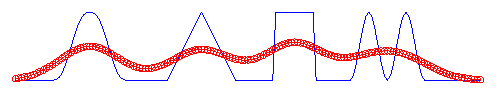
\includegraphics[width=0.5\textwidth]{conver/first}}
	\subfloat[схема Lax"--~Wendroff]{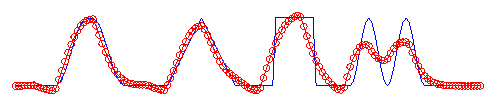
\includegraphics[width=0.5\textwidth]{conver/lw}}\\
	\subfloat[схема Beam"--~Warming]{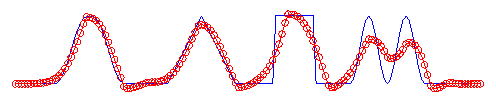
\includegraphics[width=0.5\textwidth]{conver/bw}}
	\subfloat[схема Fromm]{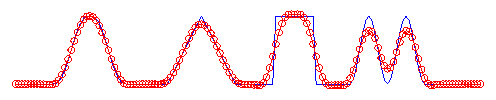
\includegraphics[width=0.5\textwidth]{conver/fromm}}\\
	\subfloat[minmod ограничитель]{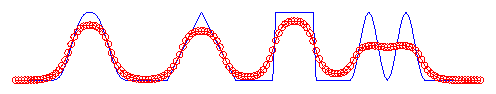
\includegraphics[width=0.5\textwidth]{conver/minmod}}
	\subfloat[van Albada ограничитель]{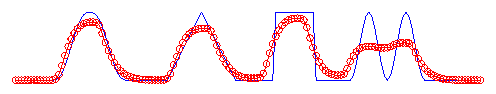
\includegraphics[width=0.5\textwidth]{conver/vanalbada}}\\
	\subfloat[Koren ограничитель]{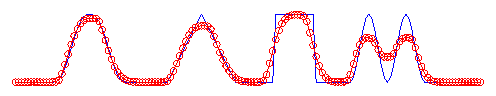
\includegraphics[width=0.5\textwidth]{conver/koren}}
	\subfloat[van Leer ограничитель]{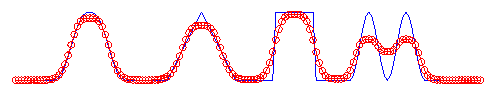
\includegraphics[width=0.5\textwidth]{conver/vanleer}}\\
	\subfloat[superbee ограничитель]{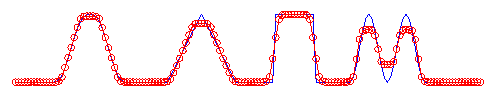
\includegraphics[width=0.5\textwidth]{conver/superbee}}
	\subfloat[MC ограничитель]{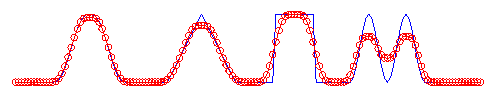
\includegraphics[width=0.5\textwidth]{conver/mc}}\\
	\subfloat[wide superbee ограничитель]{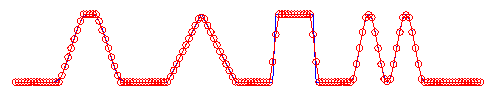
\includegraphics[width=0.5\textwidth]{conver/superbee_g}}
	\subfloat[wide third ограничитель]{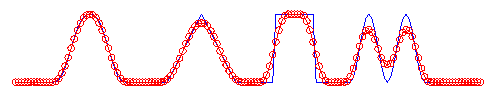
\includegraphics[width=0.5\textwidth]{conver/third_g}}\\
	\centering\subfloat[схема RK3+Koren]{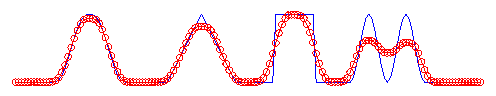
\includegraphics[width=0.5\textwidth]{conver/runge}}
	\caption{Поведение различных схем на различных решениях при числе Куранта \(\gamma=0.5\).}\label{fig:conver}
\end{figure}

Простейшая задача для сравнения ограничителей "--- это одномерная задача переноса с фиксированной скоростью без граничных условий.
На рис.~\ref{fig:conver} представлено поведение всех заявленных ограничителей при числе Куранта \(\gamma=0.5\) слева направо:
на гладком решении, с разрывом производной, разрывом самой функции и для быстро осциллирующего решения.

Сразу видно, что схема первого порядка даёт неудовлетворительные результаты, поскольку ``размазывает'' форму всех импульсов,
поэтому рекомендуется не использовать её для прецизионных расчётов.
Классические схемы (особенно \textit{Fromm}) дают неплохие результаты, однако отсутствие условия TVD влечёт за собой паразитические осцилляции,
в частности, нарушается условие неотрицательности, что особенно важно при решении кинетического уравнения,
поэтому их также стоит непригодными для использования. Отметим, что \textit{Fromm} ввиду своей симметричности лишён фазового сдвига
по сравнению с запаздывающим решением \textit{Lax"--~Wendroff} и опережающим \textit{Beam"--~Warming}.

Наихудшим среди TVD ограничителей второго порядка точности, как и ожидалось, стал \textit{minmod}.
\textit{Van Albada} также плох из-за сильной несимметричности по отношению ко знаку производной функции.
Аналогичные проблемы c ассиметричностью испытывает \textit{Koren}, который приспособлен для схемы Рунге-Кутты (формулы \ref{eq:rk1}--\ref{eq:rk2}).

Лучше всего гладкие решения аппроксимирует \textit{MC}, \textit{van Leer} и \textit{wide third} ограничители,
поскольку они (это относится и к схеме \textit{Fromm}) имеют одинаковое значение производной \(\varphi'(1)\).
Отличия обуславливаются различным поведением при больших градиентах.
Видно, что \textit{wide third} лучше сходится к экстремумам функции.
Напомним, что, кроме прочего, \textit{wide third} имеет третий порядок сходимости при любых \(\gamma\) в отличие от конкурентов
(значение \(\gamma=0.5\) выбрано специально для сравнения схем третьего порядка).

В сходимости к разрывным и быстро осциллирующим решениям с большим перевесом первенствует \textit{wide superbee},
который также по всем показателям обошел своего классического коллегу \textit{superbee}.

Для численного сравнения ограничителей использовалась октаэдрическая норма:
\begin{equation}\label{eq:norm}
	D(M) = \|f-v\| = \frac1{M}\sum_{i=1}^{M}|f_i-v_i| = \mathcal{O}(h^q),
\end{equation}
где \(v_i\) "--- точное решение, \(h\) "--- сеточный шаг, \(q\) "--- порядок сходимости, \(M\) "--- общее число ячеек.
На гладких решениях порядок сходимости при условии сходимости совпадает с порядком аппроксимации согласно теореме Лакса"--~Рябенького.
В противном случае на сегодняшний день теоретический анализ затруднителен, поэтому будем использовать экспериментальные значения.
В табл.~\ref{tab:q_value} представлены соответствующие значения порядков сходимости исследуемых схем при различных числах Куранта
для решений с разрывами значения и первых трёх производных. Они вычислялись по простой формуле
\[ q = \log_2\frac{D(M)}{D(2M)} \]
для следующих функций:
\begin{alignat*}{2}
	 g_0(x) &= 1,\quad &|x| < 1, \\
	 g_1(x) &= 1-|x|,\quad &|x| < 1, \\
	 g_2(x) &= 1-3|x|^2+2|x|^3,\quad &|x| < 1, \\
	 g_3(x) &= 1-10|x|^3+15|x|^4-6|x|^5,&\quad |x| < 1. 
\end{alignat*}
Аналогичное сравнение широкого класса численных схем можно найти в \cite{Safronov2010}.

Схема \textit{first} везде имеет первый порядок сходимости, кроме разрывных решений,
где значение \(q=0.5\) объясняется схемной вязкостью (получается в дифференциальном приближении).
Остальные схемы отчетливо проявили свой порядок на гладком решении,
поэтому в таких случаях предпочтение стоит отдать схемам третьего порядка \textit{wide third} и \textit{RK3+Koren},
однако последняя требует б\textit{о}льшего объёма вычислений.

Что касается разрывных решений, то максимальный порядок (\(q=1\)) продемострировали \textit{superbee} и \textit{wide superbee}.
Выделение класса схем с единичным порядком "--- сложная задача, но, по-видимому,
\textit{superbee} схемы представляют собой наилучшее сочетание со вторым порядком аппроксимации.

\ctable[
	caption = Порядки сходимости исследуемых схем,
	label = tab:q_value,
]{|l|c|c|c|c||c|c|c|c|}{
	\tnote{Все экспериментальные значения порядков сходимости получены при сравнении невязок для одинаковых сеток
		с числом ячеек \(N\sim10^3\), приходящихся на ненулевые значения начальной функции.
		При дальнейшем увеличении объёма расчетной сетки порядок сходимости практически не меняется, однако
		в этом случае наблюдается исключение, поскольку значение \(q(N)\) неравномерно убывает с умельчением расчётной сетки
		от \(q(16)=1.76\) до \(q(16\cdot10^3)=0.55\) и далее.
		Это связано с особенностями начальной функции \(g_1(x)\), у которой везде, где \(\exists g''_1\), \(g''_1=0\),
		а это соответствует точке \(\theta=1\), колебания возле которой приводят к значительной потере сходимости.
		Дабы не умалять достоинств \textit{wide superbee} отметим, что он вплоть до сеток с \(N\simeq2\cdot10^3\) обладает наименьшей абсолютной невязкой.}
}{
	\hline
	\multirow{2}{*}{Лимитер} & \multicolumn{4}{c||}{\(\gamma=0.5\)} & \multicolumn{4}{c|}{\(\gamma=0.9\)} \\ \cline{2-9}
	& \(\nexists f\) & \(\nexists f'\) & \(\nexists f''\) & \(\nexists f'''\) 
	& \(\nexists f\) & \(\nexists f'\) & \(\nexists f''\) & \(\nexists f'''\) \\ \hline
	first order				& 0.500 & 1.000 & 0.991 & 0.983 & 0.500 & 1.000 & 0.998 & 0.997 \\ \hline
	Lax"--~Wendroff			& 0.674 & 1.280 & 1.956 & 1.993 & 0.582 & 1.233 & 1.964 & 1.999 \\ \hline
	Beam"--~Warming			& 0.674 & 1.280 & 1.956 & 1.993 & 0.668 & 1.291 & 1.986 & 1.999 \\ \hline
	Fromm					& 0.765 & 1.505 & \color{magenta}2.520 & \color{magenta}2.950 & 0.619 & 1.282 & 1.978 & 1.998 \\ \hline
	minmod					& 0.662 & 1.325 & 1.925 & 1.982 & 0.658 & 1.322 & 1.940 & 1.990 \\ \hline
	van Albada				& 0.675 & 1.323 & 1.954 & 1.999 & 0.670 & 1.307 & 1.967 & 1.999 \\ \hline
	van Leer				& 0.747 & 1.486 & \color{magenta}2.212 & \color{magenta}2.933 & 0.707 & 1.414 & 2.033 & 2.002 \\ \hline
	Koren					& 0.667 & 1.333 & 1.964 & 2.000 & 0.660 & 1.305 & 1.967 & 2.000 \\ \hline
	MC						& 0.752 & 1.534 & \color{magenta}2.424 & \color{magenta}2.931 & 0.691 & 1.397 & 1.991 & 2.000 \\ \hline
	superbee				& \color{olive}1.000 & 1.519 & 1.933 & 2.000 & \color{olive}0.997 & 1.500 & 1.961 & 2.000 \\ \hline
	wide superbee			& \color{olive}1.000 & 1.694 & 1.933 & 2.000 & \color{olive}1.000 & \(\sim\)1.7\tmark & 1.959 & 2.000 \\ \hline
\color{magenta}	wide third	& 0.749 & 1.508 & \color{magenta}2.597 & \color{magenta}2.918 & 0.747 & 1.534 & \color{magenta}2.530 & \color{magenta}2.947 \\ \hline
\color{magenta}	RK3+Koren	& 0.753 & 1.541 & \color{magenta}2.445 & \color{magenta}2.905 & 0.751 & 1.511 & \color{magenta}2.428 & \color{magenta}2.899 \\ \hline
}

Кроме порядка сходимости основной интерес представляет также абсолютное значение невязки.
На рис.~\ref{fig:residual} показана зависимость невязки от количества ячеек \(N\), приходящихся на ненулевое значение \(f(0,x)\).
Приведены для краткости только ограничители \textit{superbee} и третьего порядка в сравнении с классическими схемами.
На гладких функциях, как и предполагалось, наименьшую невязку на мелких сетках показал \textit{wide third},
однако на грубых сетках благодаря большим антидиффузионным потокам отличный результат показывает \textit{wide superbee}.
На разрывных решениях у всех схем невязка уменьшается практически линейно.

\begin{figure}[h]
		\subfloat[гладкая функция, \(\gamma=0.5\)]{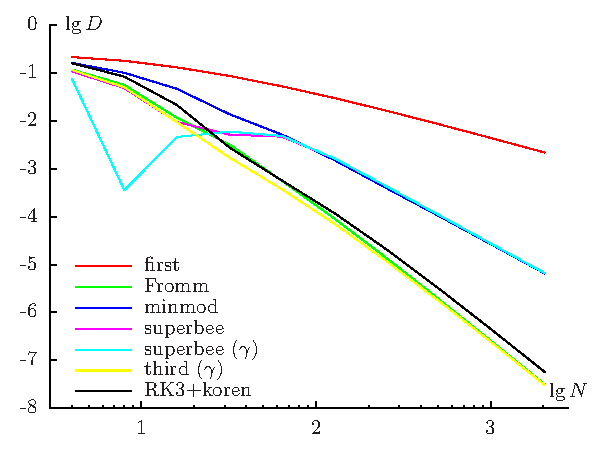
\includegraphics[width=0.5\textwidth]{residual/05_3dis.pdf}}
		\subfloat[гладкая функция, \(\gamma=0.9\)]{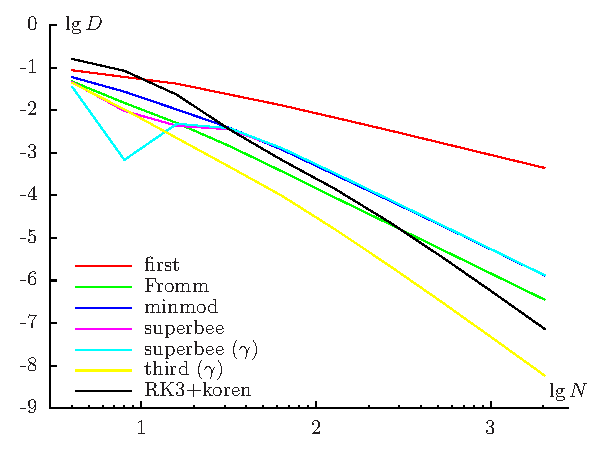
\includegraphics[width=0.5\textwidth]{residual/09_3dis.pdf}}\\
		\subfloat[разрывная функция, \(\gamma=0.5\)]{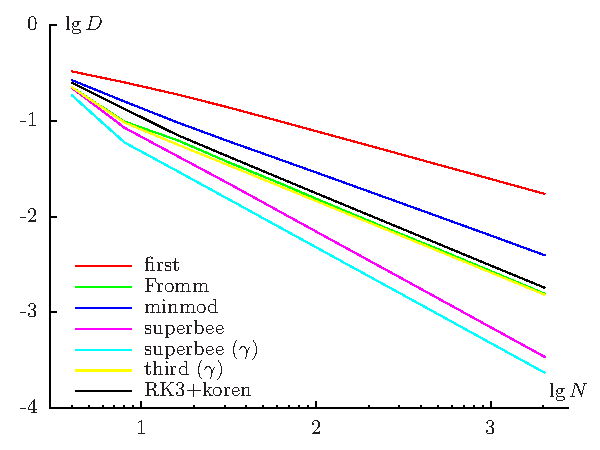
\includegraphics[width=0.5\textwidth]{residual/05_0dis.pdf}}
		\subfloat[разрывная функция, \(\gamma=0.9\)]{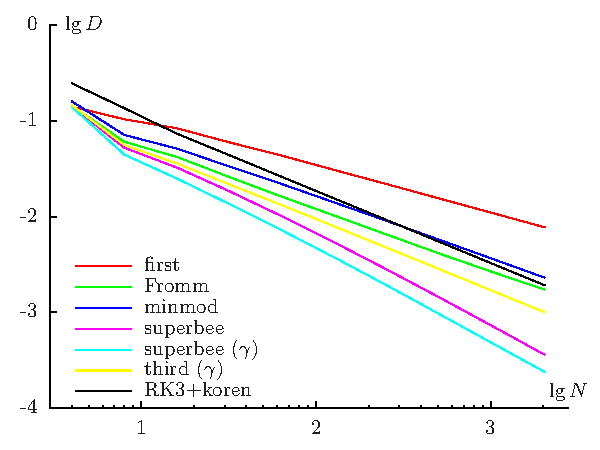
\includegraphics[width=0.5\textwidth]{residual/09_0dis.pdf}}
	\caption{Зависимость невязки от мелкости сетки.}\label{fig:residual}
\end{figure}

\section*{\centering{Заключение}}
В результате исследования можно выделить две наилучших схемы.
Для решения нестационарных задач с большими градиентами (например, в случае ударных волн)
и при использовании грубых сеток для быстрых расчётов рекомендуется использовать \textit{wide superbee}.
Наилучшую сходимость к гладким функциям (что обычно характерно для стационарных распределений) показал \textit{wide third},
что определяет его применимость для прецизионных вычислений.

\centering{\bibliographystyle{abbrv}}
\bibliography{lim,lim_rus}

\end{document}


\subsection{Интеграл столкновений. Проекционный метод дискретных ординат}
списываем у Олега

\section{Проблемно-моделирующая среда}
В настоящее время существует множество \textit{проблемно-моделирующих сред} (англ. \textit{problem solving environment}),
способных решать широкий спектр задач гидрогазодинамики.
Под ПМС понимается специализированное программное обеспечение для решения определённого класса задач,
сочетающее в себе автоматизированные вычислительные методы и пользовательский интерфейс для управления ходом решения поставленной задачи.
В качестве вычислительного метода обычно используются или численное решение уравне­ния Навье"--~Стокса
или статистическое моделирование кинетического уравнения Больцмана (метод DSMC).
Также применяются модельные уравнения, дающие верную качественную оценку только для близким к равновесным процессам.
Область явлений, для которой число Кнудсена (отношение длины свободного пробега к характерному размеру обтекаемый тел) порядка единицы,
вызывают большие сложности. Эта область наиболее характерна для моделирования газа в МЭМС и
включает в себя широкий круг явлений от теплового скольжения до затухания ударных волн. 
Для решения этой проблемы использован описанный выше консервативный метод точного решения кинетического уравнения Больцмана,
который лёг в основу разработанной ПМС.

Для достижения поставленной цели с использованием открытых технологий был написан кроссплатформенный программный код,
позволяющий эффективно выполнять расчёты как на персональном компьютере, так и на многопроцессорных кластерах.
В качестве языка программирования был выбран C++, совмещающий высокое быстродействие с объектно-ориентированным программированием,
что немаловажно для дальнейшего перспективного развития ПМС. 
Благодаря универсальности метода область решаемых задач не ограничивается описанной,
а гибкость реализации ПМС позволяет применять его не только для академических расчётов,
но и в промышленных целях для моделирования сложных конструкций.

\subsection{Общая структура}

На рис.~\ref{fig:pse} представлена схема потока данных от входных параметров, предоставляемых пользователем,
и генерации расчётной сетки до визуализации результатов с использованием специализированных пакетов.
Центральное место на рисунке занимает \textit{солвер} (или решатель) "--- программа,
выполняющая все необходимые для моделирования газа вычисления.

\begin{figure}
	\centering\footnotesize
	\begin{tikzpicture}[block/.style={shape=rectangle,rounded corners,draw=blue!50,fill=blue!20,thick,inner sep=5pt,
							minimum size=1cm,node distance=2cm,text badly centered},
						miniblock/.style={shape=rectangle,draw=blue!50,fill=blue!30,thick,inner sep=5pt,
							minimum size=1cm,node distance=5mm,text badly centered},>=latex',thick]
		\node[block,minimum width=4cm,minimum height=2.9cm] (in) at (2,1.55)			{};
		\node[block,minimum width=4cm,minimum height=2.9cm] (mesh) at (2,-1.55)			{};
		\node[block,minimum width=5.5cm,minimum height=6cm] (solver) at (7.5,0)				{};
		\node[block,minimum width=3.5cm,minimum height=6cm] (out) at (12.75,0)	{};
		\draw [<-] (in.east)+(.75cm-1pt,0) to (in.east);
		\draw [<-] (mesh.east)+(.75cm-1pt,0) to (mesh.east);
		\draw [->] (solver) to (out);

		\node[below] at (in.north) {\textbf{Входные данные}};
		\node[miniblock,text width=3.5cm,inner sep=0pt] at (2,2) {Конфигурационный XML файл};
		\node[miniblock,text width=3.5cm,inner sep=0pt] at (2,.8) {Интерактивная оболочка};

		\node[below] at (mesh.north) {\textbf{Расчетная сетка}};
		\node[miniblock,text width=3.5cm,inner sep=0pt] (rgen) at (2,-1.1) {Генератор сеток прямоугольных};
		\node[miniblock,text width=3.5cm,inner sep=0pt] (gmsh) at (2,-2.3) {GSMH};

		\node[below] at (solver.north) {\textbf{Солвер}};
		\node[miniblock,rotate=90,text width=4cm] (int) at (9.4,0) {Интеграл столкновений};
		\node[miniblock,text width=2.5cm] (rect)  at (6.5,1.5) {RectSolv};
		\node[miniblock,text width=2.5cm] (gpu)   at (6.5,0) {GPUSolv};
		\node[miniblock,text width=2.5cm] (unstr) at (6.5,-1.5) {UnstructSolv};
		\draw [<->] (int.north)+(0,1.5) to (rect.east);
		\draw [<->] (int.north) to (gpu.east);
		\draw [<->] (int.north)+(0,-1.5) to (unstr.east);

		\node[below,rotate=90] (visual) at (out.west) {\textit{Визуализация}};
		\node[above,rotate=90] at (out.east) {\textbf{Выходные данные}};
		\node[miniblock,text width=1.5cm] (gnu)  at (13,2.25) 	{Gnuplot};
		\node[miniblock,text width=1.5cm] (para) at (13,0.75) 	{Paraview};
		\node[miniblock,text width=1.5cm] (bk)   at (13,-0.75) {Bkviewer};
		\node[miniblock,text width=1.5cm] (ncl)  at (13,-2.25) {NCL};
		\draw [->] (visual.east) to[in=180,out=90] (gnu.west);
		\draw [->] (visual.south)+(0,.75) to (para.west);
		\draw [->] (visual.south)+(0,-.75) to (bk.west);
		\draw [->] (visual.west) to[in=180,out=-90] (ncl.west);

		\draw [->,dashed,thin] (rgen.east)+(0,.2) to[out=0,in=135] (rect.north);
		\draw [->,dashed,thin] (rgen.east)+(0,-.2) to[out=0,in=135] (gpu.north);
		\draw [->,dashed,thin] (gmsh.east) to[out=0,in=-135] (unstr.south);

	\end{tikzpicture}
	\caption{Схема проблемно-моделирующей среды}\label{fig:pse}
\end{figure}

Для численного решения кинетического уравнения необходимо оперировать с шестимерной функцией распределения,
что предъявляет высокие требования и к объёму оперативной памяти, и к вычислительной мощности.
Поэтому изначально солверы разрабатывались для функционирования в \textit{многопроцессорной среде}.
В задачи солвера входит численное решение уравнения Больцмана методом конечных объёмов, а также эффективное распараллеливание.
Для этого вся расчётная область делится на области (домены), каждая из которых предоставляется отдельному вычислительному узлу.
Расчёт представляет собой итерационный процесс эволюции функции распределения.
С помощью её интегрирования периодически вычисляются макропараметры, которые записываются в файлы соответствующего формата для дальнейшей визуализации.
Эффективное распараллеливание позволило, с одной стороны, значительно сократить время расчётов (с недель до часов),
с другой "--- обеспечить саму возможность прецизионного расчета на мелких сетках, которые требуют больших объёмов памяти.
На сегодняшний день солверы используют две технологии распараллеливания.
MPI (Message Passing Interface) применяется для вычислений на кластерах из обычных процессоров,
Nvidia CUDA (Compute Unified Device Architecture) "--- для расчетов на видеокартах.
Для моделирования устройств, геометрия которых состоит из прямоугольных областей, используются прямоугольные сетки.
Они используются в солверах RectSolv и GPUSolv, которые для вычислений используют обычный и графический процессор соответственно.
Для решения задач с произвольной геометрией используется солвер UnstructSolv, который оперирует с неструктурированными сетками,
генерируемые пакетом GMSH [].
Уравнение Больцмана решается методом расщепления: по очереди моделируются перенос молекул и их столкновения друг с другом.
Поскольку результат соударений молекул не зависит от пространственной конфигурации, в частности, от координатных сеток,
то все перечисленные солверы используют единый модуль, отвечающий за взятие интеграла столкновений проекционным методом [].
Для анализа полученных результатов применяются различные программные продукты.
Для наглядной визуализации потоков используется пакет NCL (NCAR Command Language) [],
с трёхмерным распределением макропараметров удобно оперировать в среде Paraview [],
которая, кроме того, обладает возможностью обработки больших объёмов данных на кластерных системах.
Для внутреннего использования применяется собственный продукт Bkviewer [], специализированный для оперативного анализа выходных данных.

\subsection{Ввод данных}
Для компьютерного моделирования, прежде всего, пользователь должен сформулировать поставленную задачу на языке, понятном для ПМС.
Для этого используется текстовый конфигурационный файл, который передаётся солверу при его запуске.
Был выбран универсальный xml формат, обеспечивающий одновременно как высокую гибкость задания всевозможных параметров расчёта,
так и ясность, удобную для чтения (или правки) структуру текста.
Такой файл может быть создан вручную, либо с помощью специальной графической интерактивной оболочки.

Конфигурационный файл разбит на множество секций, каждая из которых описывает отдельный объект:
это может быть как применяемая разностная схема или интеграл столкновений, так и моделируемая геометрия или начальные условия задачи.
Каждому объекту соответствует в солвере собственный программный модуль.
Таким образом, задание различных параметров в секции есть выбор и настройка отдельных модулей системы.
 
Все расчеты в системе ведутся в безразмерных переменных.
Это, во-первых, облегчает анализ вычислений,во-вторых, позволяет применить критерий подобия.
Например, если определяющим для физического процесса является число Кнудсена, то результаты вычислений справедливы
как для макроустройств при низком давлении, так и для микроустройств при атмосферном.
Соответственно, начальные условия задаются также в безразмерном виде.

\subsection{Расчётные сетки}
Для решения уравнения Больцмана необходимо моделирование эволюции во времени функции распределения,
которая в общем случае шестимерна по пространственным и скоростным координатам.
Это фазовое пространство покрывается соответствующими конечными сетками.

В скоростном пространстве это просто шар радиусом в несколько тепловых скоростей
(обычно это величина порядка пяти максимальных тепловых скоростей в задаче), равномерно заполненный узлами.
В пространственных координатах могут использоваться различные сетки, покрывающие любые геометрии.
В простом случае, когда геометрия состоит из прямоугольных областей, применяются прямоугольные сетки, генерируемые встроенным модулем.
Построение разностных схем высокого порядка точности значительно проще для таких сеток.
При попытке аппроксимировать искривлённые поверхности прямоугольными ячейками возникает множество трудностей,
поэтому универсальным решением является использование неструктурированных сеток.

Для генерации неструктурированных сеток используется пакет GMSH [] с открытым кодом.
В нём используется алгоритм Delaunay [], а для улучшения качества тетраэдров "--- оптимизатор из открытого пакета Netgen [].
В рамках описываемой ПМС к пространственным сеткам предъявляются следующие требования.
С одной стороны, они должны сгущаться в областях, где движение газа представляет наибольший интерес.
Это позволяет получить хорошую точность в условиях экономии вычислительных ресурсов.
С другой стороны, необходимо высокое качество ячеек (приближенность их к правильным фигурам).
Это связано с особенностями решения уравнения переноса: шаг по времени ограничен минимальной высотой ячейки.

\subsection{Внутреннее устройство солвера}

\begin{figure}
	\centering\footnotesize
	\begin{tikzpicture}[level 1 concept/.append style={sibling angle=60,level distance=4.5cm}, scale=1]
		\path[mindmap,concept color=black,text=white,minimum size=2cm]
		node[concept] {\LARGE\textbf{Солвер}}
		[clockwise from=90]
		child[concept color=green!50!black] {
			node[concept] {Listeners}
			[clockwise from=180]
			child { node[concept] {Starter} }
			child { node[concept] {Stopper} }
			child { node[concept] {Saver} }
			child { node[concept] {Logger} }
		}
		child[concept color=red,minimum size=2.5cm] { node[concept] {\textbf{Интеграл столкновений}} }
		child[concept color=blue] { node[concept] {Параметры газа} }
		child[concept color=orange] { node[concept] {Разбиение на домены} }
		child[concept color=blue] { node[concept] {Сетка \\ Граничные условия} }
		child[concept color=red,minimum size=2.5cm] { node[concept] {\textbf{Уравнение переноса}} };
	\end{tikzpicture}
	\caption{Структурная схема солвера}\label{fig:solver_structure}
\end{figure}

На рис.~\ref{fig:solver_structure} представлено модульное разбиение солвера,
а на рис.~\ref{fig:solver_algorithm} показан общий алгоритм его работы.

Солвер хранит всю информацию в массиве ячеек (\textit{cells}) и границ (\textit{boundaries}).
Набор ячеек считывается из сетки (\textit{grid}). Набор границ --- из геометрии (\textit{geometry}) и граничных условий.
Все ячейки знают про своих соседей, в т.\,ч. про соответствующие им граничные условия.
Параметры газа "--- это информация о молекулярном потенциале, степенях свободы, смесевом составе и т.\,д.

\begin{figure}
	\centering\footnotesize
	\begin{tikzpicture}[node distance=2cm,every path/.style={draw,>=latex',very thick},thick,
						block/.style={rectangle,text width=3cm,text=white,text badly centered,rounded corners,minimum height=4em}]
		\node[block,fill=blue] (init) {Считывание начальных данных};
		\node[block,fill=orange,below of=init] (decomp) {Разбиение расчетной сетки на домены};
		\node[block,fill=green!50!black,below of=decomp] (listeners) {Листенеры};
		\node[below of=listeners] (dummy) {};
		\node[block,fill=green!50!black,node distance=5cm,above left of=listeners] (save) {Сохранение результатов};
		\node[block,fill=green!50!black,node distance=5cm,above right of=listeners] (stop) {Остановка расчёта};

		\node[block,fill=red,left of=dummy, node distance=3cm] (ldiff) {Расчет уравнения переноса для \(\frac\tau2\)};
		\node[block,fill=red,right of=dummy, node distance=3cm] (rdiff) {Расчет уравнения переноса для \(\frac\tau2\)};
		\node[block,fill=red,below of=dummy] (integr) {Расчет интеграла столкновений \\ для \(\tau\)};

		\draw[->] (init) to (decomp);
		\draw[->] (decomp) to (listeners);
		\draw[->] (listeners.east) to [bend left=45] (rdiff.north);
		\draw[<-] (listeners.west) to [bend right=45] (ldiff.north);
		\draw[<-] (integr.east) to [bend right=45] (rdiff.south);
		\draw[->] (integr.west) to [bend left=45] (ldiff.south);
		\draw[->] (listeners) to [bend right=30] node[right,text width=1.2cm,text centered] {если \\ нужно} (stop.south);
		\draw[->] (listeners) to [bend left=30] node[left,text width=1.2cm,text centered] {если \\ нужно} (save.south) ;
	\end{tikzpicture}
	\caption{Алгоритмическая блок-схема солвера}\label{fig:solver_algorithm}
\end{figure}

После считывания начальных данных специализированный модуль (это может собственная подпрограмма или встроенный пакет в GMSH)
разбивает расчётную область на домены (англ. \textit{domain decomposition}), распределяя их между вычислительными узлами.
После этого начинается итерационный процесс в соответствии со схемой расщепления уравнения Больцмана.
Перед каждым временн\textit{ы}м шагом управление передаётся так называемым \textit{листенерам} (\textit{listener}),
каждый из которых отвечает за определённую функцию:
\begin{enumerate}
	\item \textit{Starter} на нулевой итерации задаёт начальные условия.
	\item \textit{Stopper} останавливает итерационный процесс в необхоимый момент времени,
		который может определяться как пользователем, так и на основе текущего распределения макропараметров.
	\item \textit{Saver} периодически сохраняет необходимые данные. В частности, это распределения макропараметров,
		которые в дальнейшем визуализируются с помощью специальных пакетов.
	\item \textit{Logger} соотвественно регистрирует совершенные действия в журнале.
\end{enumerate}


\section{Моделирование классических задач динамики разреженного газа}
Для апробации изложенного численного метода решения кинетического уравнения Больцмана
рассмотрена наиболее фундаментальная одномерная задача динамики разреженного газа "--- 
течение газа между двумя параллельными пластинами.

\begin{wrapfigure}{r}{4cm}
	\vspace{-10pt}
	\centering
	\begin{tikzpicture}[dashdot/.style={dash pattern=on .4pt off 3pt on 4pt off 3pt},
						>=latex',thick, scale=1]
		\fill[gray!20] (0,0) -- (3.6,0) -- (3.6,1.5) -- (0,1.5) -- cycle;
		\draw[dashdot] (-.2,0) -- (3.8,0);
		\draw[very thick] (0,1.5) -- (3.6,1.5);
		\draw[<->] (.7,0) -- (.7,.75) node[left] {\(\dfrac{L}{2}\)} -- (.7,1.5);
		\draw[<->] (3.2,0) node[above] {\(z\)} -- (2.4,0) -- (2.4,.8) node[right] {\(x\)};
	\end{tikzpicture}
	\vspace{-20pt}
	\caption{Схема задачи}\label{fig:parallel_plates}
	\vspace{-10pt}
\end{wrapfigure}

Расстояние между пластинами фиксировано и равно \(L\).
Коэффициент аккомодации \(\alpha=1\), что соответсвует полному диффузному отражению молекул от пластин.
Координатные оси направлены в соответствии со схемой на рис.~\ref{fig:parallel_plates}.
Изучается стационарное состояние одноатомного идеального газа.
В качестве молекулярной потенциала используется модель твердых сфер.

В зависимости от природы, действующих на разреженный газ сил, можно выделить 4 различных физических явления:

\begin{enumerate}
	\item \textit{Течение Куэтта}. Газ приводится в движение за счёт относительной скорости пластин.
		В классической газовой динамики задача ограничивается изучением тензора напряжений,
		при кинетическом рассмотрении кроме потока массы возникают также тепловые потоки,
		как вдоль пластин, так и в перпендикулярном направлении.
	\item \textit{Перенос тепла}. Вследствие разности температур пластин возникает поперечный поток тепла.
		В модели сплошной среды он пропорционален градиенту температур,
		но в пределе бесстолновительного газа он зависит только от разности температур.
	\item \textit{Течение Пуазёйля}\footnote
		{
			Поскольку ранее по типографским правилам буквы \textit{е} и \textit{ё} не различались,
			распространённым стало чтение фамилии Пуазёйль через букву \textit{е}, однако здесь мы будем придерживаться
			классической транслитерации французских слов.
		}. В этом случае возникает продольный поток газа вследствие заданного градиента давления.
		Из уравнений Навье"--~Стокса легко получается параболический профиль скоростей между пластинами.
		В разреженном газе возникает эффект \textit{скольжения} газа вдоль пластин, появляются тепловые потоки.
		Кроме того, возникает \textit{парадокс Кнудсена} "--- существование минимума потока массы в зависимости от числа Кнудсена.
	\item \textit{Тепловая траспирация} (англ. \textit{transpiration} "--- просачивание).
		Рассматривая протекание газа через неравномерно нагретые пористые вещества, Осборн Рейнольдс в 1880 году заметил [],
		что вдоль твёрдых поверхностей с градиентом температур возникает так называемое \textit{тепловое скольжение} (\textit{thermal creep}) газа.
		В это же время Джеймс Максвелл [] привел теоретическое обоснование этого явления на основе предположения,
		что неравномерное температурное распределение в газе приводит к внутренним напряжениям.
		Тепловое скольжение происходит в пристеночном слое газа толщиной порядка длины свободного пробега,
		поэтому этот эффект исчезает в гидродинамическом пределе.
\end{enumerate}

Будем рассматривать линейные приближения задач, которые соответствуют малым градиентам макропараметров.
В такой постановке они хорошо изучены для всего диапазона чисел Кнудсена, и при этом подробно табулированы с высокой точностью.
Целью моделирования является верификация проекционного метода решения кинетического уравнения Больцмана
на основе точного решения линеаризованного приближения.



\subsection{Течение Куэтта и задача переноса тепла}
\documentclass[english,russian,a4paper,12pt]{article}
\usepackage[utf8]{inputenc}
\usepackage[T2A]{fontenc}
\usepackage{babel}
\usepackage{csquotes}
% \IfFileExists{literat.sty}{\usepackage{literat}}{}

\usepackage{fullpage}
\usepackage{indentfirst}
\usepackage[font=small,labelfont=bf,labelsep=period]{caption}

\usepackage{amssymb, amsmath}
\usepackage{wrapfig}
\usepackage{graphicx}
\usepackage{movie15}

\newcommand{\dd}{\:\mathrm{d}}
\newcommand{\Kn}{\mathrm{Kn}}
\newcommand{\D}{\mathrm{d}}

\usepackage[
	pdfauthor={Rogozin Oleg},
	pdftitle={Couette Flow and Heat Transfer between Two Parallel Plates},
	colorlinks,pdftex, unicode]{hyperref}

\usepackage[
	style=alphabetic,
	language=british,
	sorting=nyt,
	url=false,
	eprint=false,
	pagetracker,
	firstinits]{biblatex}
\bibliography{couette_heat}

\title{Течение Куэтта и перенос тепла между двумя параллельными пластинами}
\author{Рогозин Олег}

\begin{document}
\maketitle
\tableofcontents

\section{Введение}

Одномерные задачи течения Ку\'{э}тта\footnote
{
	Дабы исключить неправильное произношение, приводим классическое французское произношение
	\includemovie[poster=play.png]{10pt}{10pt}{couette.mp3}
}
и переноса тепла между двумя параллельными пластинами являются наиболее простыми,
но основополагающими в динамике разреженного газа. В работе изучаются линейные приближения задач,
которые соответствуют малым градиентам макропараметров. В такой постановке они хорошо изучены
для всего диапазона чисел Кнудсена, и при этом подробно табулированы с высокой точностью.
Целью работы является верификация проекционного метода решения кинетического уравнения Больцмана
на основе точного решения линеаризованного приближения.

\section{Постановка задачи}

Рассмотрим одноатомный идеальный газ между двумя бесконечными параллельными пластинами с полным диффузным отражением.
Ось абсцисс направлена перпендикулярно пластинам, расстояние между которыми равно \(L\).
В качестве молекулярного потенциала взаимодействия выберем модель твердых сфер.

Течение Куэтта образуется при  относительном движении пластин друг относительно друга с продольной скоростью \(U\)
вдоль оси ординат, при этом плотность газа \(\rho\) и температура стенок и газа \(T\) остаются постоянными.
В стационарном состоянии уставливается константный профиль сдвигового напряжения \(p_{xy}\).

Задача переноса тепла ставится для фиксированного отношения температур покоящихся стенок \(T_1>T_2\),
при котором уставливается константный профиль теплового потока \(q_x\).

\section{Безразмерные переменные}

В работе будем придерживаться современных обозначений, принятых 
в классической монографии Соуна <<Молекулярная динамика>>~\cite{Sone2007}.
Безразмерные величины будем отмечать символом <<шляпки>>.

Микроскопические величины в уравнении Больцмана
\[
	\frac{\partial{f}}{\partial{t}} + \xi_i\frac{\partial{f}}{\partial X_i} = 
	\int (f'f'_1-ff_1)|\boldsymbol{\xi}-\boldsymbol{\xi}'|b\dd b \dd \varepsilon \boldsymbol{\dd\xi},
\]
такие как координата \(X_i\), скорость \(\xi_i\), время \(t\), прицельное расстояние \(b\)
и функция распределения \(f\) принимают безразмерный вид согласно формулам:
\[ f = \hat{f}f_0,\; \xi_i = \zeta_i\nu_0,\; X_i = x_i\ell_0,\;
	t = \hat{t}\frac{\ell_0}{\nu_0},\; b = \hat{b}d_m \]
Для макроскопических параметров, таких как плотность \( \rho = \hat{\rho}\rho_0\), макроскопическая скорость \(v_i = \hat{v}_iv_0\),
температура \(T = \hat{T}T_0\), тензор напряжений \(p_{ij} = \hat{p}_{ij}p_0\) и тепловой поток \(q_i = \hat{q}_iq_0\) 
безразмерные соотношения определим естественным образом:
\[ \rho_0 = f_0 \nu_0^3, \; v_0 = \nu_0, \; p_0 = \rho_0RT_0, \; q_0 = p_0\nu_0, \]
где \(R = k_B/m\) "--- удельная газовая постоянная, равная отношению постоянной Больцмана \(k_B\) к молекулярной массе \(m\).
Значения \(\rho_0\) и \(T_0\) выбирались как средние плотность и температура соответственно,
в частности для задачи переноса тепла \(T_0 = (T_1+T_2)/2\).

Наконец, свяжем две единицы измерения длины \(x\), \(b\) и единицы температуры \(T_0\), скорости \(\nu_0\):
\[ \ell_0 = \frac{m}{\pi\sqrt2 \rho_0 d_m^2}, \; \nu_0 = \sqrt{2RT_0}, \]
так что \(\ell_0\) окажется длиной свободного пробега, \(d_m\) "--- эффективным диаметром молекул газа,
а \(\nu_0\) "--- средней тепловой скоростью газа.

Итак, в безразмерных переменных кинетическое уравнение Больцмана примет вид
\[ \frac{\partial\hat{f}}{\partial\hat{t}} + \zeta_i\frac{\partial\hat{f}}{\partial x_i} = \hat{J}(\hat{f},\hat{f}), \]
\[ 
	\hat{J}(\hat{f},\hat{f}) = \frac1{\pi\sqrt2}\int (\hat{f'}\hat{f'_1}-\hat{f}\hat{f_1})
	|\boldsymbol{\zeta}-\boldsymbol{\zeta}'| \hat{b}\dd \hat{b} \dd \varepsilon \boldsymbol{\dd\zeta},
\]
а макропараметры будут вычиляться по формулам:
\begin{alignat*}{2}
	\hat{\rho} &= \int \hat{f}\boldsymbol{\dd\zeta}, \\
	\hat{\rho}\hat{v}_i &= \int \zeta_i \hat{f}\boldsymbol{\dd\zeta}, \\
	\frac3{2}\hat{\rho}\hat{T} &= \int(\zeta_i-\hat{v}_i)^2\hat{f}\boldsymbol{\dd\zeta}, \\
	\frac1{2}\hat{p}_{ij} &= \int(\zeta_i-\hat{v}_i)(\zeta_j-\hat{v}_j)\hat{f}\boldsymbol{\dd\zeta}, \\
	\hat{q}_i &= \int(\zeta_i-\hat{v}_i)(\zeta_j-\hat{v}_j)^2\hat{f}\boldsymbol{\dd\zeta}.
\end{alignat*}

Давление вычисляется как \(\hat{p} \equiv \hat{p}_{ii}/3 = \hat{\rho}\hat{T}\), а число Кнудсена будем определять как \(\Kn=\ell_0/L\).
Аналогично можно записать безразмерные коэффициенты вязкости \(\mu\) и теплопроводности \(\lambda\):
\[ \mu = \hat{\mu}\rho\nu\ell = \hat{\mu}\sqrt{\hat{T}}\mu_0, \; \mu_0 = \rho_0\nu_0\ell_0, \]
\[ \lambda = \hat{\lambda}R\rho\nu\ell = \hat{\lambda}\sqrt{\hat{T}}\lambda_0, \; \lambda_0 = R\rho_0\nu_0\ell_0. \]
 
\section{Методика численного решения уравнения Больцмана}

Кинетическое уравнение Больцмана решалось симметричным методом расщепления на уравнение переноса
\[ \frac{\partial\hat{f}}{\partial\hat{t}} + \zeta_i\frac{\partial\hat{f}}{\partial x_i} = 0, \]
для которого использовалась консервативная TVD схема с ограничителем третьего порядка аппроксимации,
и уравнение релаксации
\[ \frac{\partial\hat{f}}{\partial\hat{t}} = \hat{J}(\hat{f},\hat{f}), \]
которое в свою очередь решалось проекционным методом.

В качестве дискретного пространства скоростей использовался шар радиусом \(4.3\nu_0\)\footnote
{
	4.3 тепловых скорости достаточно, чтобы обеспечить точность 0.01\% совпадения
	первых тринадцати моментов функции распределения (малой величины) с соответствующими разностными аналогами.
},
равномерно заполненный узлами так, что на радиусе помещалось 16 точек.
Одномерное координатное пространство состояло как минимум из 30 одинаковых кубических ячеек,
при условии что их размер не превышал единицы.

Для взятия интеграла столкновений применялись сетки Коробова размером от 0.1 до 1 млн. точек.
Стационарные значения макропараметров усредненялись на последних 500 временных итераций,
что обеспечивало точность не ниже 0.1\%.

Для ускорения расчётов в качестве начальной функции распределения выбиралось тринадцатимоментное приближение Грэда
\[ 
	\hat{f}_{G13} = \frac{\hat\rho}{(\pi\hat T)^{3/2}}\exp\left(-\frac{c_i^2}{\hat T}\right)
	\left( 1+\frac{\hat p_{ij}c_ic_j}{\hat p\hat T} + \frac4{5}\frac{\hat q_ic_i}{\hat p\hat T}\left(\frac{c_i^2}{\hat T}-\frac5{2}\right) \right),
	\quad c_i = \zeta_i - \hat v_i
\]
с соответствующими точному решению профилями макропараметров.

В задаче Куэтта относительная скорость пластин равнялась \(\hat{U}=0.01\),
и такое же значение отношения температур \(\hat{T}_1/\hat{T}_2\) использовалось в задаче теплопереноса.
Этого достаточно, чтобы обеспечить линейность задачи с точностью порядка 0.01\%.

\section{Результаты}

\subsection{Течение Куэтта}

Для задачи Куэтта сравнивались зависимости сдвигового напряжения (рис.~\ref{fig:couette:shear}),
потоков массы (рис.~\ref{fig:couette:flow}) и тепла (рис.~\ref{fig:couette:qflow})
через половину сечения от числа Кнудсена.

В рамках линейной теории для бесстолкновительного газа
\[ \frac{\hat{p}_{xy}}{\hat{U}} = -\frac1{\sqrt{\pi}}, \]
а при небольших \(\Kn\) справедливо асимптотическое решение\footnote
{ Получается при решении уравнения Больцмана методом Грэда"--~Гильберта~\cite{Sone2007}: разложение по малому параметру \(\Kn\). }
\[ \frac{\hat{p}_{xy}}{\hat{U}} = \frac{2\hat{\mu}\Kn}{1-\sqrt{\pi}k_0\Kn}. \]
Коэффициенты вязкости \(\hat{\mu}\) и скольжения \(k_0\) для модели твёрдых сфер равны~\cite{Sone2007}
\[ \hat{\mu} = 0.562773, \; k_0 = -1.2540. \]
Отбросив знаменатель, получим гидродинамическое решение \(\hat{p}_{xy} = 2\hat{\mu}\Kn\hat{U}\).
Численные значения точного решения табулированы в~\cite{Sone1990}.

Кроме того, для сравнения представлены некоторые результаты 
решения модельного кинетического уравнения БКВ (Больцмана"--~Крука"--~Веландера).
Несмотря на хорошое совпадение модельного решения с точным для значения сдвигового напряжения,
метод БКВ даёт значительную погрешность для потоков массы и тепла~\cite{Sone1990},
поэтому нигде не приводятся соответствующих табличных значений.

\begin{figure}
	\centering
	\includegraphics{couette/graph.pdf}
	\caption{Зависимость сдвигового напряжения от числа Кнудсена}\label{fig:couette:shear}
\end{figure}

\begin{figure}
	\centering
	\includegraphics{couette/flow.pdf}
	\caption{Зависимость потока массы через половину сечения от числа Кнудсена}\label{fig:couette:flow}
\end{figure}

\begin{figure}
	\centering
	\includegraphics{couette/qflow.pdf}
	\caption{Зависимость потока тепла через половину сечения от числа Кнудсена}\label{fig:couette:qflow}
\end{figure}

На рис.~\ref{fig:couette:shear} наблюдается хорошое совпадение результатов.
Однако для бесстолкновительного газа заметно превышение \(\hat{p}_{xy}\) на 0.61\%,
что может быть обусловлено только ошибкой дискретной аппроксимации функции распределения по скоростному пространству.
При интерполяции полученной кривой на интервале \(\Kn\in[0,0.2]\) асимптотическим решением 
можно произвести подбор параметров нелинейным методом наименьших квадратов.
С его помощью в области континуального описания газа определяется оклонение 
от коэффициентов вязкости (\(+0.83\%\)) и скольжения (\(-1.2\%\)).
Если все полученные значения нормировать на точное значение для бесстолкновительного газа (разделить на 1.0061),
то погрешность в коэффициенте вязкости снижается до \(+0.22\%\), что является уже приемлимым результатом.

На рис.~\ref{fig:couette:flow},~\ref{fig:couette:qflow} для сильно разреженного газа наблюдаются
значительные отклонения, природа которых пока не определена.

\subsection{Перенос тепла}

Для задачи переноса тепла проанализируем зависимость теплового потока \(q\) от числа Кнудсена (рис.~\ref{fig:heat}).

В рамках линейной теории для бесстолкновительного газа
\[ \frac{\hat{q}_x}{\hat{T}_1-\hat{T}_2} = -\frac1{\sqrt{\pi}}, \]
а при небольших \(\Kn\) справедливо асимптотическое решение
\[ \frac{\hat{q}_x}{\hat{T}_1-\hat{T}_2} = -\frac{\hat{\lambda}\Kn}{1+\sqrt{\pi}d_1\Kn}. \]
Коэффициенты теплопроводности \(\hat{\lambda}\) и скачка температуры на стенке \(d_1\) для модели твёрдых сфер равны~\cite{Sone2007}
\[ \hat{\lambda} = 2.129475, \; d_1 = 2.4001. \]
Отбросив знаменатель, получим гидродинамическое решение \(\hat{q}_x = -\hat{\lambda}\Kn(\hat{T}_1-\hat{T}_2)\).
Численные значения точного решения табулированы в~\cite{Sone2007}.

\begin{figure}
	\centering
	\includegraphics{heat/graph.pdf}
	\caption{Зависимость теплового потока от числа Кнудсена}\label{fig:heat}
\end{figure}

Как и в задаче о течении Куэтта, на рис.~\ref{fig:heat} видна хорошая сходимость к точному решению,
однако одновременно наблюдаются те же проблемы: завышение значений теплопотока на \(0.63\)\%
для бесстолкновительного газа и значительная ошибка в коэффициенте теплопроводности (\(+2.2\%\)).
По всей видимости, последняя объясняется неточной аппроксимацией угла разлёта сталкивающихся молекул,
в частности, существованием минимально разрешимого угла.

\subsection{Исследование погрешности}

Логичным представляется исследование зависимости указанных погрешностей от числа интерполирующих узлов
скоростного пространства. Будем анализировать ошибки аппроксимации задачи переноса тепла.
Для этого коэффициент теплопроводности вычислялся локально в точке \(x_0=\hat L/2\) по формуле
\[ \hat{q_x}(x_0) = -\hat{\lambda}\frac{\D\hat T}{\D x}\bigg|_{x=x_0}. \]

Соответствующие графики в логарифмическом масштабе представлены на рис.~\ref{fig:error}.
Наклон прямых говорит примерно о квадратичной зависимости:
\[ \varepsilon \propto R_\Omega^{-2} \propto V_\Omega^{-2/3}, \]
где \(R_\Omega\) "--- число узлов на радиусе скоростной сетки, \(V_\Omega\) "--- её объём.

При \(R_\Omega = 40\) точность вычисления теплового потока повышается до \(0.1\%\),
а коэффициента теплопроводности только до \(0.5\%\).
Отклонение точки \(R_\Omega = 40\) для \(\lambda\) объясняется прямой по всей видимости 

\begin{figure}
	\centering
	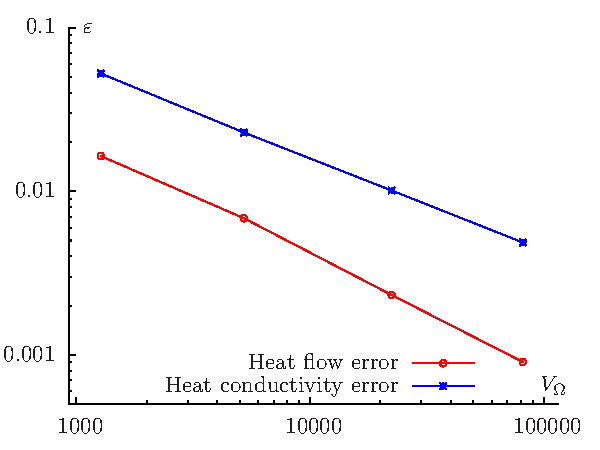
\includegraphics{error/error.pdf}
	\caption{
		Зависимость от числа узлов на радиусе скоростной сетки погрешностей вычисления 
		теплопотока для бесстолкновительного газа и коэффициента теплопроводности для слаборазреженного газа
	}\label{fig:error}
\end{figure}

\section{Заключение}

Показана удовлетворительная сходимость численного решения уравнения Больцмана проекционным методом
простейших одномерных линейных задач: течения Куэтта и переноса тепла, --- к эталонным на основе
линеаризованного уравнения.

Выявлены две проблемы. Во-первых, плохая сходимость погрешности аппроксимации теплового потока по отношению к
объёму используемой памяти. Возможным решением является корректировка всех значений макропараметров
по их отклонению в бесстолкновительном режиме при используемом \(R_\Omega\) от некоторого большего \(R_\Omega\),
при котором результаты можно считать достоверными.

Во-вторых, существенна погрешность в определении коэффициентов вязкости и особенно теплопроводности.
По всей видимости, качественно улучшить аппроксимацию межмолекулярного потенциала позволит лишь использование
более чем двухточечного проекционного метода, который обеспечит точное значение угла разлёта.

\printbibliography

\end{document}


\subsection{Течение Пуазёйля}
\newcommand{\muHS}{\hat{\mu}_{\rm{HS}}}
\newcommand{\QHS}{\hat{Q}_{\rm{HS}}}

На сегодняшний день хорошо исследована линейная задача Пуазёйля (малый градиент давления) как на основе
теоретических работ с использованием модельных кинетических уравнений~\cite{Cercignani1963, Cercignani1966, Sharipov1999},
линеаризованного уравнения Больцмана~\cite{Ohwada1989b}, а также статистического моделирования DSMС, IP~\cite{Fan2001},
так и эспериментальных~\cite{Porodnov1974, Ewart2007}.

Введём следующие обозначения. Расстояние между пластинами равно \(H\), их температура \(T_0\) постоянна.
Градиент давления приложен вдоль оси \(z\).

\subsubsection{Модель сплошной среды}

Самое простое приближение может быть получено в рамках модели сплошной среды,
которая справедлива для пренеьрежимо малых чисел Кнудсена.
На прямоугольный элемент высотой \(\D x\) и длиной \(\D z\) действуют сила внутреннего трения
\(\D F = \mu v_{xx} \D z \D x \) и гидростатическая сила \(\D F = p_z \D z \D x \).
Здесь \(\mu\) "--- вязкость газа, \(p_z = \rho_z T_0 k/m\) "--- градиент давления (температуру газа считаем везде постоянной \(T=T_0\)).
В стационарном течении сумма сил равна нулю
\begin{equation}\label{eq:forces}
	\frac{p_z}{\mu} + v_{xx} = 0. 
\end{equation}
Скорость газа у стенок равна нулю \(v(\pm H/2) = 0\), поэтому получаем квадратичное распределение:
\[ v(x) = \frac{p_z}{\mu}\frac{H^2}{8}\left(1-4\frac{x^2}{H^2}\right). \]

Для модели твёрдых сфер во втором приближении Чэпмена"--~Энскога вязкость газа равна~\cite{Chapman1991}
\[ \mu_{\rm{HS}}^{(2)} = \frac{5}{16\sqrt\pi}\frac{\sqrt{mkT}}{d_m^2}. \]
Обозначая безразмерный коэффициент вязкости как \(\muHS^{(2)}\), найдём
\[ \mu_{\rm{HS}}^{(2)} = \muHS^{(2)}\rho_0\nu_0\ell, \quad \muHS^{(2)} = \frac{5\sqrt{\pi}}{16}. \]
Для достижения большей точности в качестве коэффициента вязкости будем использовать точное значение,
вычисленное в~\cite{Pekeris1957}\footnote{
	В работе показано, что для модели твёрдых сфер интегральное уравнение Больцмана"--~Гильберта
	можно свести в дифференциальному уравнению четвертого порядка, которое уже несложно решить численно.
}:
\begin{equation}\label{eq:eta_hs}
	\mu_{\rm{HS}} = \muHS\rho_0\nu_0\ell, \quad \muHS = 1.016034\cdot\muHS^{(2)} = 0.562773.
\end{equation}
Кроме того, отметим высокую скорость сходимости разложения Чэпмена"--~Энскога\footnote
{
	В классическом учебнике \textit{Ландау Л.Д., Лифшиц Е.М.} Теоретическая физика. Т. 10. Физическая кинетика
	на стр.~53 в примечаниях к форм.~(5--6) допущена опечатка:
	сходимости для коэффициентов теплопроводности и вязкости следует поменять местами.
}:
\[ \muHS^{(3)} = 1.01485\cdot\muHS^{(2)}, \quad \muHS^{(4)} = 1.01588\cdot\muHS^{(2)} \]
Переходя к безразмерным переменным
\[
	\frac{\rho_z \nu_0 H}{\rho_0}u(x) = \frac{\rho_z\nu_0^2}{2}\:
	\frac1{\muHS\rho_0\nu_0\ell}\:\frac{H}{8}\frac{\ell}{\Kn}
	\left(1-4\frac{x^2}{H^2}\right)
\]
получаем значение скорости
\[ u(x) = \frac{\Kn^{-1}}{16\muHS} \left(1-4\frac{x^2}{H^2}\right). \]
Мы учли, что \(\rho(x)=\rho_0\) и \(H=\ell/\Kn\).
Интегрируя по \(x\) вычисляем поток массы
\[ Q_P = \frac2{H}\int\limits_{0}^{H/2} u(x) \dd x = \frac{\QHS}{\Kn}, \quad \QHS = \frac1{24\muHS}. \]

\subsubsection{Условие скольжения первого порядка}

Модель сплошной среды справедлива для \(\Kn\lessapprox10^{-2}\).
Как известно на расстоянии порядка \(\ell\) от твердой поверхности (так называемый слой Кнудсена)
состояние газа не описывается навье-стоксовым приближением.
Это выражается, прежде всего, в существовании температурного и скоростного скачков на границе газ-поверхность.
Впервые соответсвующие граничные условия для максвелловских молекул сформулировал
Джеймс Клерк Максвелл в 1879 году~\cite{Maxwell1879}.

Поскольку нас не интересуют температурные градиенты, то условие на границе примет вид:
\[ v|_{x=\pm\frac{H}{2}} \pm \frac{\mu\sqrt{\pi}}{\rho_0\nu_0}v_x|_{x=\pm\frac{H}{2}} = 0. \]
Подставляя значение вязкости из~\eqref{eq:eta_hs}, получаем
\[ v|_{x=\pm\frac{H}{2}} \pm \muHS\sqrt{\pi}\cdot\ell v_x|_{x=\pm\frac{H}{2}} = 0. \]
Разрешая уравнение~\eqref{eq:forces} для таких граничных условий, находим поперечный профиль скоростей
\[ u(x) = \frac{\Kn^{-1}}{16\muHS} \left(1-4\frac{x^2}{H^2}\right) + \frac{\sqrt{\pi}}{4}. \]
Интегрирование соответственно приводит к потоку массы
\[ Q_{1\text{slip}} = \QHS\left(\frac1{\Kn} + 6\sqrt{\pi}\muHS \right). \]

Использование описанных выше граничных условий позволяет в целом расширить область применимости
уравнений Навье"--~Стокса до \(\Kn\lessapprox10^{-1}\), однако точное решение задачи возможно
только в рамках кинетического уравнения.

\subsubsection{Решение задачи на основе модельных уравнений}

Ввиду сложности интеграла столкновений первые решения задачи Пуазёйля для широкого диапазона чисел Кнудсена
появились на основе модельных уравнений~\cite{Cercignani1963}.
Наиболее известна кинетическая модель Бхатнагара, Гросса, Крука, Веландера\footnote
{
	В литературе чаще встречается аббревиатура БГК по первым буквам авторов статьи~\cite{Bhatnagar1954},
	однако независимо примерно в то же самое время эту модель предложил Веландер~\cite{Welander1954}.
},
в которой вместо нелинейного оператора столкновения используется
\[ J(f) = \frac{f_{\rm{M}}(\boldsymbol\xi) - f(\boldsymbol\xi)}{\theta}, \]
где \(f_{\rm{M}}(\boldsymbol\xi)\) "--- максвелловская функция распределения, \(\theta\) "--- время свободного пробега.
В отличии от модели твердых сфер, где формула~\eqref{eq:eta_hs} задает среднюю длину свободного пробега молекул,
в БКВ-приближении понятие пробега фактически нельзя строго определить,
поэтому обычно используют его связь с вязкостью газа:
\[ \ell_{\rm{BKW}} = \frac{\sqrt{\pi}}{2}\theta\nu_0 = \frac{\mu\sqrt{\pi}}{\rho\nu_0}. \]
Для того чтобы сравнить результаты моделирования необходимо использовать одно и то же значение вязкости,
что обеспечивает идентичность течения в континуальном режиме.
Поэтому, положив \(\mu = \mu_{\rm{HS}}\), получим
\[ \ell_{\rm{BKW}} = \muHS\sqrt{\pi}\cdot\ell. \]

В работе~\cite{Cercignani1965} исследовано асимптотическое поведение потока массы\footnote
{
	Значения потока массы в работах \fbox{Черчиньяни} необходимо делить на 2,
	поскольку в качестве единичного потока выбрана величина \(-(\rho_z H^2 \nu_0)/2\).
}:
\[ Q_{\rm{BKW}} = \frac{\rho}{12} + \frac{\sigma}{2} + \frac{2\sigma^2-1}{2\rho}
	+ \frac2{3\rho^2}\left( \zeta + \frac{\sigma(4\sigma^2-9)}{4} \right)
	+ \mathcal{O}\left(\frac1{\rho^3}\right), \quad \rho \rightarrow \infty, \]
\[	Q_{\rm{BKW}} = -\frac1{2\sqrt{\pi}}\ln{\rho} + \mathcal{O}(1), \quad \rho \rightarrow 0, \]
где
\[ \rho = \frac{H}{\theta\nu_0} = \frac{\Kn^{-1}}{2\muHS}, \quad
	p(t) = \sqrt{\pi}\left( e^{t^2} - 2t\int_0^te^{u^2}\dd u \right), \]
\[ \sigma = \int_0^\infty\frac{\sqrt{\pi}te^{t^2}\dd t}{(p(t))^2+\pi^2t^2} = 1.01619\footnotemark, \quad
	\zeta = \int_0^\infty\frac{\sqrt{\pi}t^2e^{t^2}\dd t}{(p(t))^2+\pi^2t^2} = \frac3{2}. \]
\footnotetext{
	В~\cite{Albertoni1963} посредством семиточечной интерполяции интеграла получено значение \(\sigma = 1.01615\),
	однако точное вычисление даёт поправку в последнем знаке.
}
Преобразуем в разложение по числу Кнудсена:
\begin{align*}
 Q_{\rm{BKW}} = \frac\QHS\Kn + \frac{\sigma}2 &+ (2\sigma^2-1)\muHS\Kn + \\
	&+ \frac{6-9\sigma+4\sigma^3}{6}(2\muHS\Kn)^2 + \mathcal{O}\left(\Kn^3\right) , \quad \Kn \rightarrow 0,
\end{align*}
\[	Q_{\rm{BKW}} = \frac1{2\sqrt{\pi}}\ln{\Kn} + \mathcal{O}(1), \quad \Kn \rightarrow \infty. \]

Логарифмическая расходимость потока массы \(Q\) в свободномолекулярном режиме (\(\Kn\rightarrow\infty\))
обусловлена бесконечным поперечным сечением между пластинами.

Подробную базу данных высокой точности решения плоской задачи Пуазёйля методом БКВ можно найти в~\cite{Sone1998}.

Существенным недостатком БКВ модели принято считать фиксированное значение числа Прандтля
\[ \Pr = \frac{c_p\mu}{\varkappa} = 1, \]
однако для одноатомного газа \(\Pr = 2/3\).\footnote
{
	Для максвелловских молекул \(\Pr = 2/3\)~\cite{Maxwell1879}, для твёрдых сфер \(\Pr = 0.660694\)~\cite{Pekeris1957},
	эксперимент также даёт \(\Pr \approxeq 2/3\).
}
Для коррекции числа Прандтля часто используют эллипсоидную статистическую модель (ЭС)~\cite{Holway1963,Holway1966}.
Суть её в замене максвелловского распределения анизотропным трехмерным гауссовским:
\[ f_{\rm{ES}} = \frac{\rho}{\sqrt{\pi\det\mathbf{A}}}\exp\left(-\sum\limits_{i=1}^{3}\sum\limits_{j=1}^{3} A_{ij}c_ic_j \right), \]
\[ \mathbf{A} = \|A_{ij}\| = \left\|\frac{\rho_{ij}}{\Pr} - \frac{2p_{ij}}{p}\frac{1-\Pr}{\Pr} \right\|^{-1}. \]

Как показано в работе~\cite{Cercignani1966}, значения потока массы в плоской задаче Пуазёйля в БКВ и ЭС моделях 
связаны следующим соотношением:
\[ Q_{\rm{ES}}(\Kn,\Pr) = Q_{\rm{BKW}}\left(\frac\Kn\Pr\right) + \QHS\frac{1-\Pr}{\Kn}. \]

Также весьма распространённой является S-модель~\cite{Shakhov1968},
где максвелловская функция корректируется следующим образом:
\[ f_{\rm{S}} = f_{\rm{M}} \left( 1+\frac8{5}(1-\Pr)\frac{\bf{qc}}{\rho}\left(\mathbf{c}^2-\frac5{2}\right) \right) \]
Некоторые результаты решения линеаризованной задачи Пуазёйля с помощью этой модели можно найти в~\cite{Sharipov1999},
однако они практически идентичны решению кинетического уравнения БКВ.

\subsubsection{Условие скольжения второго порядка}

В настоящее время актуальной является проблема определения коэффициентов скольжения высокого порядка.
Это, во-первых, позволяет расширить область применения уравнений Навье"--~Стокса в переходном режиме.
Во-вторых, члены второго порядка моделируют минимум потока массы от числа Кнудсена (так называемый парадокс Кнудсена).

Классическая форма граничных условий второго порядка записывается как
\[ u|_w = A_1\ell u_x|_w - A_2\ell^2 u_{xx}|_w,  \]
где \(|_w\) означает значение у плоской поверхности.
В таком случае выражение для потока массы примет вид
\[ Q_{2\text{slip}} = \QHS\left(\frac1{\Kn} + 6A_1 + 12A_2\Kn\right). \]

Существует множество работ с различными оценками коэффициентов скольжения,
некоторые из которых представлены в табл.~\ref{tab:slip}.
Кроме прямых численных методов применяется также вариационный подход,
требующий гораздо меньше вычислительных ресурсов, но ограниченный по точности выбором пробной функции.

\begin{table}[h]
	\centering
	\caption{Коэффициенты скольжения}\label{tab:slip}
	\begin{tabular}{l|c|c|c}
		Автор		& Год	& \(A_1\) & \(A_2\) \\
		\hline
		Максвелл \cite{Maxwell1879} (макс. мол.)		& 1879	& 0.9975 (\(=\muHS\sqrt{\pi}\)) & 0  \\
		Черчиньяни \cite{Cercignani1965} (числ. БКВ)	& 1965	& 1.1438 (\(=\muHS2\sigma\)) & 0.6656  \\
		Оувада и др. \cite{Ohwada1989a} (числ. ТС)		& 1996	& 1.1113 (\(=\frac{\sqrt{\pi}}{2}\cdot1.25401\)) &  \\
		Черчиньяни и др. \cite{Cercignani2010} (вар. ТС)& 2010	& 1.1209 & 0.2335 \\
	\end{tabular}
\end{table}

\subsubsection{Экспериментальные данные}

По всей видимости, последние наиболее точные экспериментальные измерения потока газа в плоской задаче Пуазёйля
выполнены в работе~\cite{Ewart2007}. Высота \(H\), ширина \(w\) и длина \(L\) прямоугольного канала
соотносятся примерно как 1:50:1000 соответственно. При пятикратном отношении давлений \(P_1/P_2 = 5\) на концах канала
такой эксперимент должен достаточно описываться линейной теорией для \(\Kn\lessapprox10\)
(отношение давлений на длине свободного пробега порядка \(10^{-2}\)).
На модель плоской задачи можно уверенно опираться при \(\Kn\lessapprox1\), поскольку
при б\textit{о}льших числах Кнудсена вклад в проводимость газа вносит конечность ширины канала.

Существенными стоит отметить следующие два положения.
Во-первых, измерения проводились для гелия, для которого в большей мере справедлив молекулярный потенциал Леннарда-Джонса.
Во-вторых, кремниевые стенки канала по оценкам с помощью модели БКВ имели коэффициент аккомодации примерно \(\alpha=0.90\).

Опишем процедуру обезразмеривания экспериментальных данных.
Использовалось табличное значение из~\cite{Kestin1984} для коэффициента вязкости гелия
\[ \mu_{\rm{He}} (20^{\circ} \rm{C}) = 1.973\cdot10^{-5}\pm0.3\%\: \text{Па\(\cdot\)с}. \]
Поскольку все измерения проводились в температурном интервале \( 20-24^{\circ} \rm{C}\),
то коэффициент вязкости с высокой точностью можно вычислять по формуле
\[ \mu(T) = \mu(T_0)\sqrt{\frac{T}{T_0}}. \]
Из формулы~\eqref{eq:eta_hs} получаем эффективное сечение \(\pi d_m^2\),
которое используем для нахождения числа Кнудсена
\[ \Kn = \frac{m}{\pi\sqrt{2}\rho H d_m^2} = \frac1{\muHS}\frac{\mu_{\rm{He}}}{\rho H\nu_0} \]

Поток массы обезразмериваем с учётом конечности ширины канала:
\[ Q = \frac{F}{-\rho_z H^2 \nu_0 w} = \frac{F}{\frac{P_1-P_2}{L}\frac{\mu}{RT} H^2 \nu_0 w}, \]
где \(\mu = 4.0026\cdot10^{-3}\: \text{кг\(\cdot\)м\({}^{-3}\)}\) "--- молярная масса гелия,
\(R = 8.3143\: \text{Дж\(\cdot\)моль\({}^{-1}\)\(\cdot\)К\({}^{-1}\)} \) "--- универсальная газовая постоянная.

\subsubsection{Решение задачи на основе проекционного метода}

Далее течение Пуазёйля рассматривается на основе прямого численного решения уравнения Больцмана
проекционным методом дискретных ординат\footnote
{
	На сегодняшний день уже существуют публикации~\cite{Aristov2009}, в которых к задаче Пуазёйля применялся проекционный метод,
	однако они носят скорее ознакомительный характер.
}.
В качестве молекулярного потенциала используется модель твердых сфер,
поэтому полученные результаты будут сходится к значениям в работе~\cite{Ohwada1989b}.
В связи существованием точного решения линейной задачи Пуазёйля нашей целью будет не достижение высокой точности результатов,
а решение задачи в общей нелинейной постановке (для конечной длины канала и конечного градиента давления).
Поэтому ограничимся верификацией 2--3 знаков и выявлению необходимых требований к параметрам расчётов
в зависимости от числа Кнудсена для получения достаточной точности:
1) размеру скоростной сетки, 2) мелкости координатной сетки, 3) объёму кубатурной сетки Коробова.

\subsubsection{Общая двумерная постановка задачи}

В связи с вышесказанным будем решать двумерную задачу (несмотря на одномерность линейной задачи)
с малым, но конечным градиентом давления.

Прежде всего покажем, при каких условиях полученные результаты для канала длиной \(L\)
будут соответствовать решению линейной задачи Пуазёйля.
Обозначим плотность газа на концах канала как \(\rho_1\equiv\rho(-L/2)\), \(\rho_2\equiv\rho(L/2)\).
Считая распределение плотности линейным \(\rho_z = (\rho_2-\rho_1)/L \equiv \Delta\rho/L\),
среднее значение плотности будет находиться в центре канала \(\rho_0\equiv\rho(0) = (\rho_2+\rho_1)/2\)

Плотность газа \(\rho\), а вместе с ней и число Кнудсена изменяются вдоль оси \(z\),
но поскольку газ не адсорбируется на стенках, то поток газа должен оставаться постоянным вдоль канала \(F_L=const\).
Проинтегрируем его по всей длине \(L\), считая что поток газа в поперечном сечении равен решению линейной задачи \(F(\rho)\):
\[ \int_{-L/2}^{L/2}F_L\rho_z\dd z \equiv F_L\rho_zL = \int_{\rho_1}^{\rho_2} F(\rho)\dd\rho. \]
Будем рассматривать малые градиенты плотности, поэтому разложим правую часть в ряд по малому параметру \(\Delta\rho\):
\[ F_L = F(\rho_0) + F''(\rho_0) \frac{\Delta\rho^2}{24} + \mathcal{O}(\Delta\rho^4) \]
Тогда можно выполнить следующую оценку ошибки вычисления потока массы:
\[ \frac{\Delta F}{F} = \left|\frac{F''(\rho_0)}{F(\rho_0)}\right|\frac{\Delta\rho^2}{24}. \]
Асимптотическое исследование
\[ F(\rho\rightarrow\infty) \propto \rho \Rightarrow F''(\rho\rightarrow\infty) \propto \rho^{-3}, \]
\[ F(\rho\rightarrow0) \propto \ln\rho \Rightarrow F''(\rho\rightarrow0) \propto \rho^{-2}, \]
позволяет говорить о хорошей сходимости для малых \(\Kn\) (\(\rho\rightarrow\infty\)) и о расходимости при больших \(\Kn\).

Поскольку нам заранее известно решение задачи, то мы можем дать численные оценки.
Планка относительной ошибки в 1\% при \(\Delta\rho/\rho = 0.2\) достигается при \(\Kn \approxeq 5\).
Для \(\Kn=10\) она возрастает до 4\%.

Также следует наложить условие на минимальное значение \(L\). Из физических соображений очевидно, что
для моделирования бесконечно длинного канала необходимо, чтобы каждая молекула много раз столкнулась со
стенками канала. Поэтому основную сложность представляют большие значения \(\Kn\). Можно было бы удовлетвориться
условием \(L \gg \ell\), но в таком случае пришлось бы иметь дело с очень большими координатными сетками,
поэтому разумным представляется решение задачи для нескольких последовательно увеличивающихся длин канала и
дальнейшая оценка сходимости полученных данных.

Наконец, третьим немаловажным аспектом является формирование стационарной разности давлений и профиля скоростей.
Для этого необходимо смоделировать бесконечно большие резервуары с разным давлением по обоим концам канала.
Прямое решение этой задачи опять же приводит в большим затратам памяти.

Приемлимые результаты даёт следующий алгоритм.
В качестве граничных условий на концах канала используется максвелловское распределение с фиксированными давлением и температурой,
а макроскопическая скорость выбирается равной текущему значению в граничной ячейке.
Однако в этом случае всё-таки необходимо выбирать достаточно длинный канал,
чтобы успели релаксировать к стационарному значению высшие моменты функции распределения.\footnote
{
	Лучшей аппроксимации, а, следовательно, дальнейшего уменьшения необходимой длины канала можно добиться,
	если вместо максвелловского распределения использовать тринадцатимоментное распределение Грэда.
}

\subsubsection{Сравнение результатов}

\begin{figure}[ht]
	\centering
	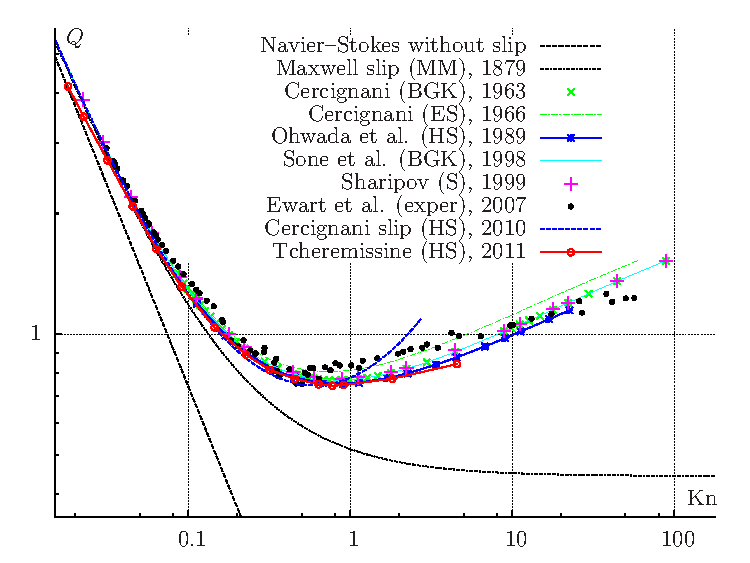
\includegraphics{problems/poiseuille.pdf}
	\caption{Зависимость потока массы \(Q\) от числа Кнудсена \(\Kn\).}\label{fig:graph}
\end{figure}

На рис.~\ref{fig:graph} представлены результаты решения задачи Пуазёйля описанными ранее методами.
Видно, что для линейной задачи модельные уравнения в общем дают близкие значения к истинным.
Экспериментальные данные также хорошо ложатся на теоретическую кривую,
несмотря на описанные выше приближения (модель твёрдых сфер с полным диффузным отражением).
Что касается значений, полученных проекционным методом при решении двумерной задачи,
то они в переходном режиме достаточно плотно прилегают к результатам численного решения Оувады и др.~\cite{Ohwada1989b},
на основании чего можно заключить о высокой точности проекционного метода.

Для малых чисел Кнудсена отклонение кривой объясняется неточной аппроксимацией межмолекулярного потенциала
на грубой скоростной сетке (радиусом 10 узлов и 3.4 тепловых скоростей).
Для сильно разреженного газа также наблюдается заниженное значение потока по этой же причине,
однако посредством образования выделенных пространственных направлений потока газа.

Таким образом, наилучшие результаты при малых вычислительных затратах проекционный метод показывает для переходного режима.
Для слабо разреженного газа необходимо, во-первых, использовать большие кубатурные сетки Коробова из-за большого шага по времени,
кроме того кинетический подход подразумевает использование размера координатной ячейки не более длины свободного пробега,
посколько это характерный размер существенных изменений функции распределения.
Вычислительные трудности для сильно разреженного газа связаны в основном с необходимостью в мелкой скоростной сетке
и в достаточном отношении длины канала к его ширине.

\subsubsection{Резюме}

Проекционным метод показал хорошую сходимость для переходного режима в двумерной геометрии,
полученные результаты совпали как с экспериментальными данными, так решением данной задачи другими численными методами.
В двумерной геометрии наблюдается б\textit{о}льшие трудности при моделировании сильно разреженного газа
ввиду характерного для методов дискретных ординат так называемого \textit{эффекта луча}:
дискретность скоростной сетки обуславливает выделенные направления движения газа в физическом пространстве.


\subsection{Тепловое скольжение и насосы Кнудсена}
\input{knudsen}

\end{document}
